%!TEX TS-program = xelatex
%!TEX encoding = UTF-8

\documentclass[twoside]{CUGThesis}

\title{基于混合权重模型的奥运项目评估与预测系统设计}
\author{何艺鸣}
\date{\today}
\school{数学与物理学院}
\classnum{信息与计算科学}
\stunum{20221003056}
\instructorone{李民}
\instructoronelevel{教授}

\usepackage{makecell,multicol,multirow,booktabs,graphicx,subcaption,float}
\captionsetup[sub]{margin=0pt}
\usepackage[hidelinks]{hyperref}
\usepackage{amsmath,amssymb}
\usepackage{algorithm,algorithmic}
\usepackage{tikz,setspace}

\newcommand{\tabincell}[2]{\begin{tabular}{@{}#1@{}}#2\end{tabular}}

\begin{document}
\maketitle
\makestatement

\begin{cnabstract}{AHP-EWM混合权重；奥运项目评估；多准则决策；六维指标体系；熵权法}
奥林匹克运动会的项目选择直接影响全球体育运动的发展方向。当前奥运项目的评估主要依赖专家委员会的主观判断，缺乏系统化的定量决策工具。本研究基于HiMCM 2024大赛提供的76个奥运项目百年历史数据，结合层次分析法与熵权法，构建了一种AHP-EWM混合权重评估模型。首先，建立包含流行度、性别平等、可持续性、包容性、创新性、安全性的六维评价指标体系。其次，通过层次分析法计算主观权重、熵权法计算客观权重，采用线性加权组合得到混合权重。然后，利用12个代表性奥运项目的历史数据验证模型有效性，定量分析了三种权重方法的差异。最后，对2032年布里斯班奥运会进行预测分析，推荐电子竞技、板球、匹克球作为重点候选项目。实验结果表明，混合权重模型能够综合主客观信息，在组合系数$\alpha=0.5$时排名结果稳定，可为国际奥委会的项目筛选决策提供科学依据。
\end{cnabstract}

\begin{enabstract}{AHP-EWM hybrid weight; Olympic event evaluation; multi-criteria decision making; six-dimensional indicator system; entropy weight method}
The selection of Olympic sports directly influences the global development of athletics. Current evaluation primarily relies on subjective expert committees, lacking systematic quantitative tools. Based on the HiMCM 2024 dataset covering 76 Olympic sports over a century, this study develops an AHP-EWM hybrid weight evaluation model. First, a six-dimensional indicator system is established encompassing popularity, gender equity, sustainability, inclusivity, innovation, and safety. Second, AHP computes subjective weights and EWM computes objective weights, combined via linear weighting. Using 12 representative Olympic sports for validation, the model recommends esports, cricket, and pickleball as top candidates for the 2032 Brisbane Olympics. Results show the hybrid model effectively integrates subjective and objective information with stable rankings at $\alpha=0.5$, providing scientific support for IOC decision-making.
\end{enabstract}

\makeToc

\begin{spacing}{2}\section{绪论}\end{spacing}

\subsection{研究背景}

奥林匹克运动会作为全球最具影响力的体育盛会，其项目设置不仅关乎竞技层面的公平性，更直接影响着全球体育运动的发展方向和资源分配\cite{Li2013}。近年来，奥运项目的评估与调整进入了一个前所未有的活跃期：2020年东京奥运会新增攀岩、冲浪、滑板等项目，2024年巴黎奥运会首次引入霹雳舞，而2028年洛杉矶奥运会又将加入板球、腰旗橄榄球等新兴项目。与此同时，空手道在2020年完成奥运首秀后随即被排除出2024年的赛程，棒球和垒球则经历了多次进出循环。这些频繁的变动表明，国际奥委会正积极寻求在保持传统与拥抱创新之间找到平衡点。

国际奥委会在《奥林匹克2020+5议程》中明确提出了15项改革建议\cite{IOC2023}，涵盖增强奥运独特性与普遍性、促进可持续发展、加强与年轻观众的数字化互动、鼓励虚拟运动与电子竞技发展等方面。这些改革方向进一步表明，奥运项目的选择需要更加科学化、系统化、可量化，而非仅仅依赖经验判断。

然而，当前的奥运项目评估主要依赖专家委员会的主观经验和定性讨论，缺乏系统化、可量化的决策工具。这种传统方法存在若干固有的局限性。其一，专家意见存在明显的个体差异：不同背景的专家可能对同一项目的价值做出截然不同的判断，缺乏统一的标准使得最终的决策难以形成广泛共识。其二，评估标准相对模糊，决策过程的透明度不足，外界难以追溯某个项目入选或淘汰的具体依据。其三，历史数据中包含的大量统计信息——如项目的参赛连续性、设项规模的增长趋势、在不同国家和文化背景下的普及程度——在当前评估体系中未能得到充分利用。Song等\cite{Song2025}也指出，奥运项目的选择过程具有内在主观性，霹雳舞入选2024巴黎奥运却未入选2028洛杉矶奥运即为典型案例。

为克服上述难题，需要一套可获取、有历史纵深的数据作为支撑，并借助系统的定量方法辅助决策。本研究基于HiMCM大赛提供的奥运项目历史数据集，从中提取了76个运动小项自1896年至2028年的设项数序列，经过数据清洗、缺失值识别和趋势统计等预处理工作后，为每个运动构建了涵盖参赛届数、设项规模、增长趋势和历史稳定性等多个层面的特征指标。在此基础上，结合层次分析法\cite{Saaty2007}与熵权法\cite{Wang2019}，构建AHP-EWM混合权重评估模型，旨在为奥运项目的定量评估提供一种科学、透明且可复现的方法框架。

\subsection{研究意义}

\subsubsection{理论意义}

本研究将多准则决策方法应用于奥运项目评估这一特定领域，创新性地采用了层次分析法与熵权法相结合的混合权重模型\cite{Zhang2023,Liang2023}。这一方法具有双重理论贡献。一方面，它为体育决策科学化提供了新的研究范式：传统的体育管理研究主要依赖经验总结和定性分析，而本研究展示了如何将专家经验通过AHP结构化为可量化的权重，同时利用EWM从数据中提取客观信息，使决策过程兼具理论严谨性和实践可操作性。另一方面，本研究建立了涵盖流行度、性别平等、可持续性、包容性、创新性、安全性六个维度的评价指标体系，丰富了奥运项目管理理论，为后续研究者提供了可借鉴的方法论框架和指标设计思路。

\subsubsection{实践意义}

本研究的成果可直接应用于多个实践场景，具有较为广泛的应用价值。首先，为国际奥委会提供一套定量化的项目评估工具，辅助其在项目筛选过程中做出更加科学、透明且可追溯的决策，减少单纯依靠主观判断所带来的不确定性。其次，为各国奥委会的项目申办提供数据驱动的决策支持，帮助其识别具有竞争优势的候选项目并制定更具针对性的申办策略。此外，为各国际体育联合会的项目推广提供策略参考，使其能够根据评估结果有针对性地提升项目的竞争力。最后，本研究的模型框架也可作为体育管理教育的教学案例，促进量化分析方法在体育人才培养中的推广和应用。

\subsection{国内外研究现状}

\subsubsection{多准则决策方法研究}

多准则决策是决策科学的重要分支，主要研究在多个相互冲突的准则下如何选择最优方案。在实际决策中，不同指标的相对重要性往往难以直接比较，因此需要一种系统化的方法将定性判断转化为定量权重。Saaty\cite{Saaty2007}提出的层次分析法（AHP）正是为此而生。该方法通过构建两两比较的判断矩阵，将决策者的主观经验以1-9标度的形式量化，再通过特征值求解得到各指标的权重向量，为复杂决策问题提供了一套完整的分析框架。然而，纯AHP方法完全依赖专家的主观判断，当专家经验不足或意见分歧较大时，权重的可靠性会受到一定影响。

熵权法（EWM）则从另一个角度切入：它基于信息熵理论，通过评估各指标在方案间的变异程度来确定权重\cite{Wang2019}。EWM的核心逻辑是：某个指标在不同方案之间差异越大，说明该指标包含的决策信息越丰富，其权重应相应较高。这种数据驱动的方法完全避免了主观判断的干扰，但其局限在于可能忽略领域知识——数据上差异大的指标不一定在决策意义上更重要。

考虑到AHP与EWM各自的优势和不足，将两者结合形成混合权重模型成为一种自然的选择。近年来，AHP与EWM的组合应用已成为多准则决策研究中的一个热点方向。Zhang等\cite{Zhang2023}在煤矿动力灾害风险评估中将AHP与EWM结合模糊综合评价，通过16个二级指标构建了评估体系，验证了混合权重相比传统单一方法具有更高的准确性和可靠性。Liang等\cite{Liang2023}将AHP-EWM应用于矿区治理模型选择，通过定量分析克服了传统方法主观性过强的缺陷，并论证了三层指标体系下混合权重的稳定性。Chen等\cite{Chen2016}在福建省农业气象灾害风险区划中采用AHP-EWM方法，结合GIS技术将灾害风险进行了空间可视化，进一步拓展了该方法的应用场景。Shang等\cite{Shang2009}在城市土地集约利用评价中运用熵权法对AHP权重进行改进，确定了组合权重并讨论了具体评价步骤。Hou和Huang\cite{Hou2010}则将熵权层次分析模型应用于旅游地社区参与度评价，验证了混合方法在社会经济领域的适用性。上述研究表明，综合主客观信息的混合决策方法在各个领域均展现出优于单一方法的性能。

\subsubsection{奥运项目评估研究}

专门针对奥运项目评估的量化研究目前尚处于起步阶段，但已有的工作为本研究提供了重要的基础。国际奥委会对新项目的评估标准涵盖流行度、性别平等、可持续性、包容性、创新性、安全性六个维度，这六个维度共同构成了一个初步但尚未完全定量化的指标体系。李凤梅\cite{Li2013}从人文取向、经济价值、社会属性等角度系统分析了奥运项目的设置标准，提出了以社会性为导向推动项目创新、以经济性为动力促进项目推广、以人文性为理念控制项目规模的三项改革原则，为指标体系的构建提供了理论支撑。

在量化评估方法方面，Song等\cite{Song2025}的研究是目前最具参考价值的直接相关工作。他们提出了一个基于AHP评分、PCA特征提取和KNN分类器的奥运项目选择框架，对电子竞技、澳式足球、匹克球等2032年布里斯班奥运会的候选项目进行了预测分析。该研究验证了定量方法在奥运项目评估中的可行性，但其重心在于分类（入选/淘汰）而非评分排序。此外，其权重的确定仅依赖于AHP方法，未引入客观数据对权重进行修正。本研究在Song等的基础上做出两个关键改进：一是引入EWM提供数据驱动的客观权重，与AHP的主观权重形成互补；二是由分类问题转向评分排序问题，为IOC提供更精细化的量化结果。

\subsection{研究内容与方法}

\subsubsection{研究内容}

本研究围绕奥运项目评估问题展开，主要包括以下五个方面的内容。第一，构建六维评价指标体系。该体系涵盖流行度、性别平等、可持续性、包容性、创新性、安全性六个维度，每个维度下设若干子指标，形成两层指标结构。指标体系的建立是后续一切定量分析的基础，决定了评估的全面性和针对性。第二，设计AHP与EWM相结合的混合权重计算方法。该方法分别利用AHP从专家判断中提取主观权重、利用EWM从数据中提取客观权重，再通过线性加权组合得到混合权重，从而综合主观经验与客观数据两方面的优势。第三，利用HiMCM历史数据和IOC官方报告对模型进行验证。通过12个代表性项目的评分排名与实际奥运决策的对比，检验模型的有效性和准确性。第四，开发评估系统与可视化模块，将理论模型转化为可操作的软件工具，使用户能够直观查看权重分布、评分排名和灵敏度分析结果。第五，对2032年布里斯班奥运会的潜在新增项目进行预测分析，展示模型在真实决策场景中的应用价值。

\subsubsection{研究方法}

本研究综合运用了文献研究、实证分析和系统开发三类方法。在文献研究阶段，通过系统梳理AHP、EWM及奥运评估相关领域的理论成果和应用案例，为模型构建奠定了理论基础。在实证分析阶段，以HiMCM数据集和IOC官方数据为基础，对构建的混合权重模型进行数值验证和灵敏度分析，评估其在实际数据上的表现。在系统开发阶段，基于Python实现了完整的权重计算、评分排序和可视化功能，将理论成果转化为可操作的软件工具。

\subsection{论文组织结构}

本文共分六章，按照理论推导、实验验证、系统实现的逻辑逐步展开。第一章为绪论，介绍研究背景、研究意义和国内外研究现状，明确研究内容和总体框架。第二章为理论基础与文献综述，系统阐述AHP、EWM、混合权重模型以及奥运项目评估的相关理论和方法。第三章为混合权重评估模型构建，详细推导模型的形式化定义、六维指标体系、主客观权重的计算方法以及混合权重的组合策略。第四章为实验设计与数据分析，利用实际数据对模型进行验证，并对2032年奥运项目进行预测。第五章为系统设计与实现，介绍评估系统的架构设计和核心模块实现。第六章为总结与展望，归纳研究的主要发现和创新点，指出研究的不足和未来改进方向。


\begin{spacing}{2}\section{理论基础与文献综述}\end{spacing}

\subsection{多准则决策理论概述}

多准则决策是指在多个相互冲突的准则下，从有限或无限方案中选择最优方案的决策过程。在实际决策中，几乎没有哪个重要问题可以仅凭单一准则做出判断，因此如何在不同准则之间进行权衡成为决策科学的核心问题。多准则决策方法主要分为两类。多属性决策（MADM）从有限且离散的方案集合中选择最优方案，适用于方案明确、数量有限的场景，如供应商选择、投资项目评估等。多目标决策（MODM）则在连续方案空间中寻找满意解，通常涉及约束条件下的多目标优化问题。本研究属于多属性决策范畴——奥运项目评估本质上就是从一组明确的候选项目中，基于多个评价准则选出综合表现最优的项目组合。

\subsection{层次分析法}

\subsubsection{基本原理}

层次分析法由Saaty\cite{Saaty2007}于20世纪70年代提出，是一种将复杂决策问题层次化、定量化的系统分析方法。其核心思想是将决策问题分解为三个层次：目标层（解决问题的总体目标）、准则层（影响决策的各类因素）、方案层（待选的具体方案），然后通过两两比较的方式确定各层元素之间的相对重要性，最终得到各方案在总体目标下的优先排序。这种层次化分解的优势在于：它将一个复杂的、难以直接量化的决策问题转化为一系列简单的两两比较问题，从而降低了决策的认知负担，提高了判断的一致性和可靠性。在本研究中，目标层是"评估奥运项目的综合竞争力"，准则层是流行度、性别平等、可持续性等六个维度，方案层则是各候选运动项目。

\subsubsection{判断矩阵}

对于$n$个指标，构造判断矩阵$A = [a_{ij}]_{n \times n}$，其中$a_{ij}$表示指标$i$相对于指标$j$的重要性。判断矩阵满足以下互反性质：
\begin{equation}
a_{ij} > 0, \quad a_{ji} = 1/a_{ij}, \quad a_{ii} = 1
\label{eq:reciprocal}
\end{equation}

$a_{ij}$的取值并非随意指定，而是需要遵循一套标准化的标度体系。Saaty提出1至9标度法来量化比较结果，如表\ref{tab:scale}所示。这一标度体系的设计考虑了人类心理认知的极限——心理学研究表明，人在同一时间内最多能有效区分7$\pm$2个不同的等级，因此9级标度是合理且实用的选择。例如，若一个决策者认为"流行度"比"安全性"明显重要，则$a_{12}=5$，相应地$a_{21}=1/5$。

\begin{table}[htbp]
\centering
\caption{萨蒂1-9标度法\cite{Saaty2007}}
\label{tab:scale}
\begin{tabular}{cl}
\toprule
标度 & 含义 \\
\midrule
1 & 同等重要 \\
3 & 稍微重要 \\
5 & 明显重要 \\
7 & 强烈重要 \\
9 & 极端重要 \\
2,4,6,8 & 中间值 \\
\bottomrule
\end{tabular}
\end{table}

\subsubsection{权重计算}

判断矩阵构造完成后，需要通过数学方法从中提取权重向量。最常用的方法是求解特征值问题：
\begin{equation}
AW = \lambda_{\max} W
\label{eq:eigenvalue}
\end{equation}
其中$\lambda_{\max}$为矩阵$A$的最大特征值，$W$为对应的特征向量。对$W$进行归一化处理后即得到各指标的权重向量。这一方法的几何直观是：在理想情况下，如果判断矩阵是完全一致的（即$a_{ij} \cdot a_{jk} = a_{ik}$对任意$i,j,k$成立），则权重向量精确等于最大特征值对应的特征向量。

\subsubsection{一致性检验}

在实际决策中，由于人的判断难以完全一致，构建的判断矩阵往往存在一定程度的不一致性。例如，决策者可能认为$A > B$且$B > C$，但同时又给出了$A < C$的判断。为了衡量这种不一致的程度，需要定义一致性指标和一致性比率：
\begin{equation}
CI = \frac{\lambda_{\max} - n}{n - 1}, \quad CR = \frac{CI}{RI}
\label{eq:consistency}
\end{equation}

其中$RI$为平均随机一致性指标，其取值通过大量随机模拟获得，如表\ref{tab:ri}所示\cite{Saaty2007}。$CI$衡量了$\lambda_{\max}$与$n$的偏离程度——当判断矩阵完全一致时，$\lambda_{\max} = n$，此时$CI=0$。$CR$则将$CI$与同阶随机矩阵的$RI$进行对比，$CR < 0.1$意味着不一致性在可接受的范围内，判断矩阵通过一致性检验；若$CR \ge 0.1$，则需要重新审视和调整判断矩阵中的比较值。

\begin{table}[htbp]
\centering
\caption{随机一致性指标$RI$}
\label{tab:ri}
\begin{tabular}{cccccccc}
\toprule
$n$ & 3 & 4 & 5 & 6 & 7 & 8 & 9 \\
\midrule
$RI$ & 0.52 & 0.89 & 1.12 & 1.26 & 1.36 & 1.41 & 1.46 \\
\bottomrule
\end{tabular}
\end{table}

\subsection{熵权法}

\subsubsection{信息熵概念}

信息熵是香农信息论中度量不确定性的核心概念，反映了系统的无序程度或信息的平均不确定性。信息熵的数学定义为：
\begin{equation}
H(X) = -\sum_{i=1}^{n} p_i \ln p_i
\label{eq:entropy_def}
\end{equation}
其中$p_i$为系统处于状态$i$的概率。从定义可以看出：当系统中某一状态的概率为1（其他状态概率为0）时，$H=0$，表示系统完全没有不确定性；当所有状态等概率分布时，$H$达到最大值，此时系统的不确定性最大。在多准则决策的背景下，这一性质具有重要的方法论意义：如果一个指标在各方案之间的取值差异很大（即信息熵小），说明该指标能够有效区分不同方案，因此应赋予更高的权重；反之，如果某指标在所有方案上的取值几乎相同（即信息熵接近最大值），则该指标对决策几乎没有贡献，权重应相应降低。

\subsubsection{熵权计算}

对于决策矩阵$X = [x_{ij}]_{n \times m}$（$n$个方案，$m$个指标），熵权计算分为四个步骤。第一步为数据标准化。由于不同指标的量纲和取值范围可能不同，需要先将原始数据映射到统一的$[0,1]$区间。正向指标（越大越好）采用以下标准化方式：
\begin{equation}
\tilde{x}_{ij} = \frac{x_{ij} - \min_i x_{ij}}{\max_i x_{ij} - \min_i x_{ij}}
\label{eq:normalize}
\end{equation}

负向指标（越小越好）则采用反向标准化：
\begin{equation}
\tilde{x}_{ij} = \frac{\max_i x_{ij} - x_{ij}}{\max_i x_{ij} - \min_i x_{ij}}
\label{eq:neg_normalize}
\end{equation}

第二步计算各指标下各方案的比重$p_{ij} = \tilde{x}_{ij} / \sum_i \tilde{x}_{ij}$。第三步计算各指标的信息熵：
\begin{equation}
H_j = -\frac{1}{\ln n} \sum_{i=1}^n p_{ij} \ln p_{ij}
\label{eq:info_entropy}
\end{equation}

除以$\ln n$是为了将熵值归一化到$[0,1]$区间，便于不同指标之间的比较。第四步计算熵权：
\begin{equation}
w_j = \frac{1 - H_j}{\sum_{j=1}^m (1 - H_j)}
\label{eq:entropy_weight}
\end{equation}

其中$D_j = 1 - H_j$称为信息效用值，表示第$j$个指标对决策的贡献程度。$D_j$越大，说明该指标包含的有效信息越多，相应的熵权也越大。这一方法的优势在于完全数据驱动，不依赖任何主观判断，但需要注意的是，它可能放大数据噪声的影响。

\subsection{混合权重模型}

\subsubsection{组合权重的必要性}

AHP权重和EWM权重从不同角度反映了指标的相对重要性：前者体现的是专家经验和领域知识的积累，后者揭示的是数据本身的结构特征。两种方法各有不可替代的优势，但也存在各自的局限性。纯AHP方法的权重完全取决于专家的主观判断，当专家团队构成不均衡、经验有限或存在利益冲突时，权重可能偏离客观实际。纯EWM方法虽然避免了主观偏差，但完全从数据出发，可能将数据噪声误判为有效信息，同时也无法融入重要的领域知识。例如，某项运动的安全性数据在各运动之间差异很小（导致EWM赋予较低的权重），但从IOC的角度来看，安全性却是一个必须优先考虑的维度。因此，将两种方法结合形成混合权重模型，能够在保留各自优势的同时弥补彼此的不足，是一种更为稳健和合理的权重确定策略\cite{Zhang2023,Shang2009}。

\subsubsection{线性组合模型}

线性组合模型是将主观权重与客观权重进行加权平均的最简形式：
\begin{equation}
W = \alpha \cdot W^{AHP} + (1 - \alpha) \cdot W^{EWM}
\label{eq:hybrid}
\end{equation}
其中$\alpha \in [0,1]$为组合系数，控制主客观权重的相对贡献。当$\alpha = 0.5$时，主客观权重被等权对待；当$\alpha > 0.5$时，模型更倾向于专家的主观判断；当$\alpha < 0.5$时，模型更依赖数据的客观分布。$\alpha$的选择本质上反映了决策者对专家经验和客观数据的信任程度，这种灵活性使得模型能够适应不同的决策情境和数据条件。

\subsubsection{组合系数确定}

组合系数的确定方法主要有三种。经验法最为直接，取$\alpha = 0.5$作为默认值，其合理性在于既不偏向主观也不偏向客观，是一种中立的起点选择。灵敏度分析法通过测试不同$\alpha$取值（如从0.1到0.9以0.1为步长）下评估结果的变化情况，观察哪些指标和排名对$\alpha$敏感、哪些相对稳定，从而确定一个稳健的$\alpha$区间。优化法则基于历史数据，通过最小化预测误差或最大化与实际决策的一致性来拟合最优$\alpha$值，但这种方法需要足够的历史决策数据作为训练集。本研究综合使用经验法和灵敏度分析法：首先采用$\alpha = 0.5$作为基准值进行实验，然后在实验章节中通过灵敏度分析验证该取值下的结果稳定性\cite{Zhang2023,Liang2023}。

\subsection{奥运项目评估相关研究}

\subsubsection{国际奥委会评估标准}

国际奥委会在对新项目进行评估时，主要从六个维度进行综合考量\cite{Li2013}。流行度是核心指标之一，关注项目的观众收视率、社交媒体讨论度和全球参与人数，反映了该运动在公众中的影响力和吸引力。性别平等关注男女运动员的参赛比例是否均衡，以及是否存在混合项目，这与IOC推动性别平等的长期战略高度一致。可持续性评估项目的环境影响，包括碳排放水平、场馆建设需求、设备资源消耗等，这与《奥林匹克2020+5议程》中强调的可持续发展目标直接对应。包容性衡量项目与残奥会的关联程度，以及其在发展中国家和不同文化背景中的普及情况，体现了奥林匹克运动对多样性的追求。创新性反映项目的年轻化程度和技术革新能力，近年新引入的攀岩、滑板、霹雳舞等项目都具有鲜明的创新性特征。安全性则从运动员的受伤风险和医疗保障需求出发进行评价，是保障体育公平竞争和运动员健康的基本前提。这六个维度共同构成了一个较为全面但尚未完全定量的评估框架，本研究正是在此框架基础上构建量化的指标体系。

\subsubsection{现有方法对比}

现有奥运项目评估方法各有特点，如表\ref{tab:method_compare}所示。传统专家评议方法虽然经过长期的实践检验，但其主观性过强、缺乏量化依据的问题一直存在。Song等\cite{Song2025}提出的AHP-PCA-KNN方法在量化评估方面迈出了重要一步，但其侧重于分类任务（将项目划分为"高/中/低"三个优先级类别），而非提供连续的评分排名。本研究的AHP-EWM混合权重模型则在评分排序方面具有优势，能够为每个项目提供一个连续的综合评分，便于决策者进行更精细化的比较和排序。

\begin{table}[htbp]
\centering
\caption{奥运项目评估方法对比}
\label{tab:method_compare}
\begin{tabular}{lccc}
\toprule
方法 & 主观性 & 客观性 & 适用场景 \\
\midrule
传统专家评议 & 高 & 低 & 定性决策 \\
AHP-PCA-KNN\cite{Song2025} & 中 & 高 & 分类问题 \\
本研究AHP-EWM混合模型 & 中 & 中 & 评分排序 \\
\bottomrule
\end{tabular}
\end{table}

本研究的方法与现有研究的区别不仅体现在技术路线上，更体现在应用场景的不同定位。现有方法更适合在项目生命周期的初期进行筛选决策，即判断某项目应该"入选"还是"淘汰"；而本研究的混合权重模型则适用于更精细化的评估场景，例如在已确定某项目基本符合入选条件后，需要进一步量化其在各个维度上的表现水平和整体竞争力，为后续的资源分配和政策调整提供依据。


\begin{spacing}{2}\section{混合权重评估模型构建}\end{spacing}

\subsection{问题数学化建模}

\subsubsection{多准则决策问题定义}

为建立精确的数学模型，首先需要将奥运项目评估问题形式化地表述为一个多准则决策问题。设候选项目集合为$S = \{s_1, s_2, \ldots, s_n\}$，评价指标集合为$C = \{c_1, c_2, \ldots, c_6\}$，其中每个$c_j$对应六维指标体系中的一个维度（流行度、性别平等、可持续性、包容性、创新性、安全性）。对于每个项目$s_i$，其在每个指标$c_j$上的原始表现为$x_{ij}$，从而构成决策矩阵$X = [x_{ij}]_{n \times 6}$。

问题的核心目标可以表述为：确定一组权重向量$W = (w_1, w_2, \ldots, w_6)$，满足归一化条件$\sum_{j=1}^6 w_j = 1$且$w_j \ge 0$，使得基于这些权重计算得到的综合评分$v_i$能够合理、准确地反映各项目的相对优劣程度。权重的确定是评估模型的核心环节，直接决定了最终评估结果的质量和可信度。

\subsubsection{综合评分模型}

在权重向量确定之后，综合评分采用加权求和的方式进行计算：
\begin{equation}
v_i = \sum_{j=1}^{6} w_j \cdot E_{ij}
\label{eq:score}
\end{equation}

其中$E_{ij}$是项目$i$在维度$j$上的归一化综合值。需要特别说明的是，$E_{ij}$并非原始数据$x_{ij}$，而是经过两层处理后的结果：首先，各子指标在维度内部通过EWM进行加权综合，得到该维度的原始综合值；然后，对该原始综合值进行归一化处理，得到最终的$E_{ij}$。这两层处理的目的在于消除不同量纲和量级对综合评分的影响，使得最终的加权和能够公平地反映各项目在不同维度上的表现。权重的确定则是整个评估模型的核心环节，本文将采用AHP与EWM相结合的方式来确定$W$，具体方法将在后续小节中详细阐述。

\subsection{六维评价指标体系}

基于国际奥委会评估标准\cite{IOC2023}和相关研究\cite{Li2013,Song2025}，构建六维评价指标体系。表\ref{tab:indicators}详细说明了各维度的含义、衡量要素和数据来源。

\begin{table}[htbp]
\centering
\caption{六维评价指标体系}
\label{tab:indicators}
\begin{tabular}{cllc}
\toprule
编号 & 指标 & 说明 & 数据来源 \\
\midrule
$c_1$ & 流行度 & 设项数规模、增长趋势、参赛届数占比 & HiMCM数据 \\
$c_2$ & 性别平等 & 男女参赛比例均衡度 & IOC报告\cite{IOC2024} \\
$c_3$ & 可持续性 & 参赛连续性、设项数稳定性、韧性 & HiMCM数据 \\
$c_4$ & 包容性 & 跨时代程度、分支项目数 & HiMCM+IPC\cite{IPC2024} \\
$c_5$ & 创新性 & 首次入奥时间距今年数、近年变化率 & HiMCM数据 \\
$c_6$ & 安全性 & 受伤率反向评分 & 医学文献\cite{Song2025} \\
\bottomrule
\end{tabular}
\end{table}

每个维度下设置若干子指标，形成两层指标体系。第一层为六维主指标，反映项目在不同宏观方面的表现；第二层为各维度下的细分指标，提供更具体的量化依据。以流行度维度为例，其子指标包括：该运动的总参赛届数（反映长期持续的受欢迎程度）、设项数历史增长率（反映受欢迎程度的变化趋势）、近三届奥运会的设项规模（反映当前受欢迎程度）等。可持续性维度的子指标则包括最大连续参赛届数（反映参赛的稳定性）、设项数的变异系数（反映设项规模的波动程度）以及是否曾经历过淘汰后回归（反映项目的韧性）。这种两层结构既保证了评估的全面性——六维主指标从不同侧面覆盖了影响奥运项目价值的各类因素，又赋予了模型处理异构数据的能力——不同维度的子指标可以根据数据的可获得性独立调整，某一维度的子指标变化不会影响其他维度的计算。

\subsection{层次分析法主观权重}

\subsubsection{判断矩阵构建}

在AHP方法的实际应用中，判断矩阵的构建通常依赖领域专家的知识。本研究基于奥林匹克运动项目评估的通用标准，构建了五位不同背景的模拟专家（包括体育管理学者、奥运研究专家、体育经济学研究者、体育行政管理人员和国际体育研究学者）对六维指标进行两两比较的数据。每位专家根据1-9标度法独立给出判断矩阵，各专家的权重偏好向量如表\ref{tab:expert_profiles}所示。然后通过几何平均法将五个矩阵整合为一个综合判断矩阵，从而消除个体差异带来的偏差。

\begin{table}[htbp]
\centering
\caption{五位模拟专家的权重偏好设定}
\label{tab:expert_profiles}
\begin{tabular}{lcccccc}
\toprule
专家 & 流行度 & 性别平等 & 可持续性 & 包容性 & 创新性 & 安全性 \\
\midrule
A（体育管理学者） & 0.396 & 0.194 & 0.091 & 0.075 & 0.043 & 0.201 \\
B（奥运研究专家） & 0.310 & 0.237 & 0.102 & 0.091 & 0.077 & 0.183 \\
C（体育经济学研究者） & 0.456 & 0.114 & 0.088 & 0.108 & 0.096 & 0.138 \\
D（体育行政管理人员） & 0.272 & 0.216 & 0.151 & 0.085 & 0.085 & 0.191 \\
E（国际体育研究学者） & 0.366 & 0.189 & 0.097 & 0.085 & 0.036 & 0.227 \\
\bottomrule
\end{tabular}
\end{table}

专家A作为体育管理学者，认为流行度和安全性是最关键的评估维度（权重分别0.396和0.201），反映了竞技体育管理中对公众关注度和运动员保障的双重重视。专家B作为奥运研究专家，偏好相对均衡，性别平等权重提升至0.237，体现了其对IOC性别平等战略的认同。专家C作为体育经济学研究者，赋予流行度极高的权重（0.456），符合经济学视角下"受众规模决定价值"的逻辑。专家D作为体育行政管理人员，权重分布最为均匀，各维度差异较小，体现了管理实务中全面权衡的特点。专家E作为国际体育研究学者，安全性权重达0.227，反映了对运动员健康和风险管理的高度关注。

每位专家的判断矩阵分别通过一致性检验（$CR < 0.1$），其几何平均整合后的综合判断矩阵如式\eqref{eq:jm_full}所示。

\begin{equation}
A = \begin{bmatrix}
1.000 & 1.644 & 3.677 & 4.338 & 5.404 & 2.000 \\
0.608 & 1.000 & 1.888 & 1.888 & 2.605 & 1.000 \\
0.272 & 0.530 & 1.000 & 1.149 & 1.888 & 0.574 \\
0.231 & 0.530 & 0.871 & 1.000 & 1.320 & 0.488 \\
0.185 & 0.384 & 0.530 & 0.758 & 1.000 & 0.308 \\
0.500 & 1.000 & 1.741 & 2.048 & 3.245 & 1.000
\end{bmatrix}
\label{eq:jm_full}
\end{equation}

以矩阵第一行为例：流行度与性别平等的比较值为1.644（介于同等重要和稍微重要之间），与可持续性的比较值为3.677（介于稍微重要和明显重要之间），与包容性的比较值为4.338（明显重要），与创新性的比较值为5.404（介于明显重要和强烈重要之间），与安全性的比较值为2.000（介于同等重要和稍微重要之间）。这些比较值反映了该领域的一种共识：流行度是奥运项目评估中最重要的指标，其次是性别平等和安全性，而创新性在当前评估框架中的优先级相对较低。

\subsubsection{多专家矩阵整合}

几何平均法是整合多专家判断矩阵的常用方法，它能够有效综合多位专家的意见，同时保持判断矩阵的互反性质：
\begin{equation}
\bar{a}_{ij} = \left( \prod_{l=1}^{k} a_{ij}^{(l)} \right)^{1/k}
\label{eq:geomean}
\end{equation}

选择几何平均而非算术平均的原因在于：几何平均能够更好地保持判断矩阵的互反性。如果采用算术平均，即$\bar{a}_{ij} = \frac{1}{k}\sum a_{ij}^{(l)}$，则无法保证$\bar{a}_{ji} = 1/\bar{a}_{ij}$自动成立，需要进行额外的归一化处理。而几何平均天然满足这一性质：$\bar{a}_{ji} = (\prod a_{ji}^{(l)})^{1/k} = (\prod 1/a_{ij}^{(l)})^{1/k} = 1/(\prod a_{ij}^{(l)})^{1/k} = 1/\bar{a}_{ij}$。

\subsubsection{权重计算与一致性检验}

整合后的判断矩阵$A$通过求解特征值问题$AW = \lambda_{\max} W$得到权重向量。具体地，将最大特征值$\lambda_{\max}$对应的特征向量进行归一化处理，即得到AHP主观权重向量$W^{AHP}$。计算得$\lambda_{\max} = 6.017$，$CI = 0.003$，查表得$RI(6) = 1.26$，一致性比率$CR = 0.003 < 0.1$，判断矩阵通过一致性检验。

$\lambda_{\max} = 6.017$非常接近矩阵阶数$n=6$，表明判断矩阵的一致性很好。$CR = 0.003$远小于0.1的阈值，说明五位专家的判断在整合后保持了良好的内部一致性。

\subsubsection{模拟专家权重结果}

基于上述判断矩阵求解得到的AHP主观权重如表\ref{tab:ahp_weights}所示。流行度以0.362的权重位居首位，其次是性别平等（0.189）和安全性（0.189），这三项合计占比74.0\%，构成了评估框架的核心。可持续性（0.106）、包容性（0.090）和创新性（0.064）的权重相对较低，合计占比26.0\%。这一权重分布的特征与奥运项目评估的实际情况相符：IOC在决策中最关注的是项目的全球影响力和普及程度（即流行度），其次是性别平等和安全性这两个涉及公平竞赛和运动员权益的维度。值得注意的是，性别平等和安全性获得了相同的权重（0.189），这与近年来IOC在《奥林匹克2020+5议程》中同时强调性别平等和运动员安全保障的政策导向一致。

\begin{table}[htbp]
\centering
\caption{AHP主观权重}
\label{tab:ahp_weights}
\begin{tabular}{cccc}
\toprule
指标 & 权重 & 排名 \\
\midrule
流行度 & 0.362 & 1 \\
性别平等 & 0.189 & 2 \\
安全性 & 0.189 & 2 \\
可持续性 & 0.106 & 4 \\
包容性 & 0.090 & 5 \\
创新性 & 0.064 & 6 \\
\bottomrule
\end{tabular}
\end{table}

\subsection{熵权法客观权重}

\subsubsection{数据标准化}

EWM计算的第一步是对原始数据进行标准化处理。正向指标（如流行度、性别平等、包容性、创新性——这些维度的得分越高越好）采用式\eqref{eq:normalize}进行标准化，负向指标（如安全性——受伤率越低越安全，或者可持续性——资源消耗越少越可持续）采用式\eqref{eq:neg_normalize}进行反向标准化。以12个代表性项目的六维指标数据作为输入，经过标准化后得到一个值域为$[0,1]$的无量纲决策矩阵，为后续的熵值计算做好准备。

\subsubsection{信息熵与权重计算}

在标准化决策矩阵的基础上，依次计算比重矩阵$p_{ij}$、各指标的信息熵$H_j$、信息效用值$D_j$和熵权$w_j^{EWM}$，计算结果如表\ref{tab:ewm_weights}所示。

\begin{table}[htbp]
\centering
\caption{EWM客观权重}
\label{tab:ewm_weights}
\begin{tabular}{cccc}
\toprule
指标 & 信息熵$H_j$ & 效用值$D_j$ & 权重$w_j^{EWM}$ \\
\midrule
流行度 & 0.868 & 0.132 & 0.218 \\
性别平等 & 0.940 & 0.060 & 0.100 \\
可持续性 & 0.935 & 0.065 & 0.108 \\
包容性 & 0.895 & 0.105 & 0.174 \\
创新性 & 0.821 & 0.179 & 0.297 \\
安全性 & 0.937 & 0.063 & 0.104 \\
\bottomrule
\end{tabular}
\end{table}

从EWM的结果可以看出几个重要的现象。首先，创新性的信息熵最低（0.821），说明各运动项目在创新性维度上的表现差异最大——从传统项目如田径（创新性得分低）到新兴项目如电子竞技（创新性得分极高），差异非常显著，因此EWM赋予了创新性最高的权重（0.297）。其次，性别平等的信息熵最高（0.940），说明大多数运动项目在该维度上的得分趋于接近，这与近几届奥运会推动性别平等的努力有关——IOC的政策使得各运动项目的男女参赛比例日益均衡。再次，流行度的信息熵居中（0.868），说明各运动项目在流行度上的差异处于中等水平，EWM对其权重评价为0.218，低于AHP的0.362，体现了两种方法的不同侧重点。

\subsubsection{两层熵权计算结构}

本研究采用两层熵权计算结构来充分发挥EWM的优势。第一层计算六维主指标的权重，这是与AHP权重进行混合组合的部分，反映的是各个宏观维度对整体评估的贡献大小。第二层计算各维度内部子指标的权重，采用纯EWM法确定，反映的是每个维度下哪些子指标对该维度的区分度贡献更大。以流行度维度为例，其子指标可能包括总参赛届数（反映长期连续的热度）、设项数历史增长率（反映热度变化趋势）和近三届奥运会的设项规模（反映当前热度水平），EWM会根据这些子指标在12个项目之间的变异程度自动分配其权重。这种两层结构的优势在于：顶层保留了与AHP进行知识融合的可能性，底层则充分利用了数据驱动方法的客观性，使模型能够灵活适应不同数据类型和质量条件下的评估需求。

\subsection{混合权重组合}

\subsubsection{线性组合模型}

混合权重采用线性加权方式组合：
\begin{equation}
W = \alpha \cdot W^{AHP} + (1 - \alpha) \cdot W^{EWM}
\label{eq:hybrid_weight}
\end{equation}

取$\alpha = 0.5$，得到混合权重如表\ref{tab:hybrid_weights}所示。

\begin{table}[htbp]
\centering
\caption{AHP、EWM与混合权重对比}
\label{tab:hybrid_weights}
\begin{tabular}{lccc}
\toprule
指标 & AHP权重 & EWM权重 & 混合权重 \\
\midrule
流行度 & 0.362 & 0.218 & 0.290 \\
性别平等 & 0.189 & 0.100 & 0.144 \\
可持续性 & 0.106 & 0.108 & 0.107 \\
包容性 & 0.090 & 0.174 & 0.132 \\
创新性 & 0.064 & 0.297 & 0.181 \\
安全性 & 0.189 & 0.104 & 0.146 \\
\bottomrule
\end{tabular}
\end{table}

\subsubsection{混合权重的数学性质}

混合权重$W = \alpha W^{AHP} + (1-\alpha)W^{EWM}$具有三个重要的数学性质，这些性质保证了混合权重的合理性和实用性。（1）有界性：对于任意$\alpha \in [0,1]$，混合权重$w_j$的取值严格介于主观权重$w_j^{AHP}$和客观权重$w_j^{EWM}$之间。这一性质保证了混合权重不会偏离主客观权重太远，从而在理论上保持了与专家经验和数据信息的一致性。（2）单调性：当$\alpha$增大时，混合权重会逐渐向$W^{AHP}$方向移动；当$\alpha$减小时，则会向$W^{EWM}$方向移动。这一性质使得决策者可以通过调节$\alpha$来体现对主观经验和客观数据的不同倾向性。（3）凸组合性质：由于$\sum w_j^{AHP} = 1$且$\sum w_j^{EWM} = 1$，对于任意$\alpha$，有$\sum w_j = \alpha \cdot 1 + (1-\alpha) \cdot 1 = 1$，即归一化条件自动满足，无需额外处理。

\subsubsection{组合系数确定}

本研究推荐组合系数$\alpha = 0.5$，即主观权重与客观权重等权组合。选择这一取值主要基于以下考虑：首先，在没有充分的先验信息表明主观或客观方法更优的情况下，等权组合是一种自然且公正的选择；其次，$\alpha = 0.5$在已有文献中是最常用的取值，具有广泛的认可度\cite{Zhang2023,Liang2023}；最后，通过后续的灵敏度分析可以验证$\alpha = 0.5$附近的排名稳定性，从而为这一选择提供实证支撑。在实际应用中，决策者可以根据对专家经验和客观数据的不同信任程度，在$[0,1]$范围内灵活调整$\alpha$的取值。

\begin{figure}[htbp]
\centering
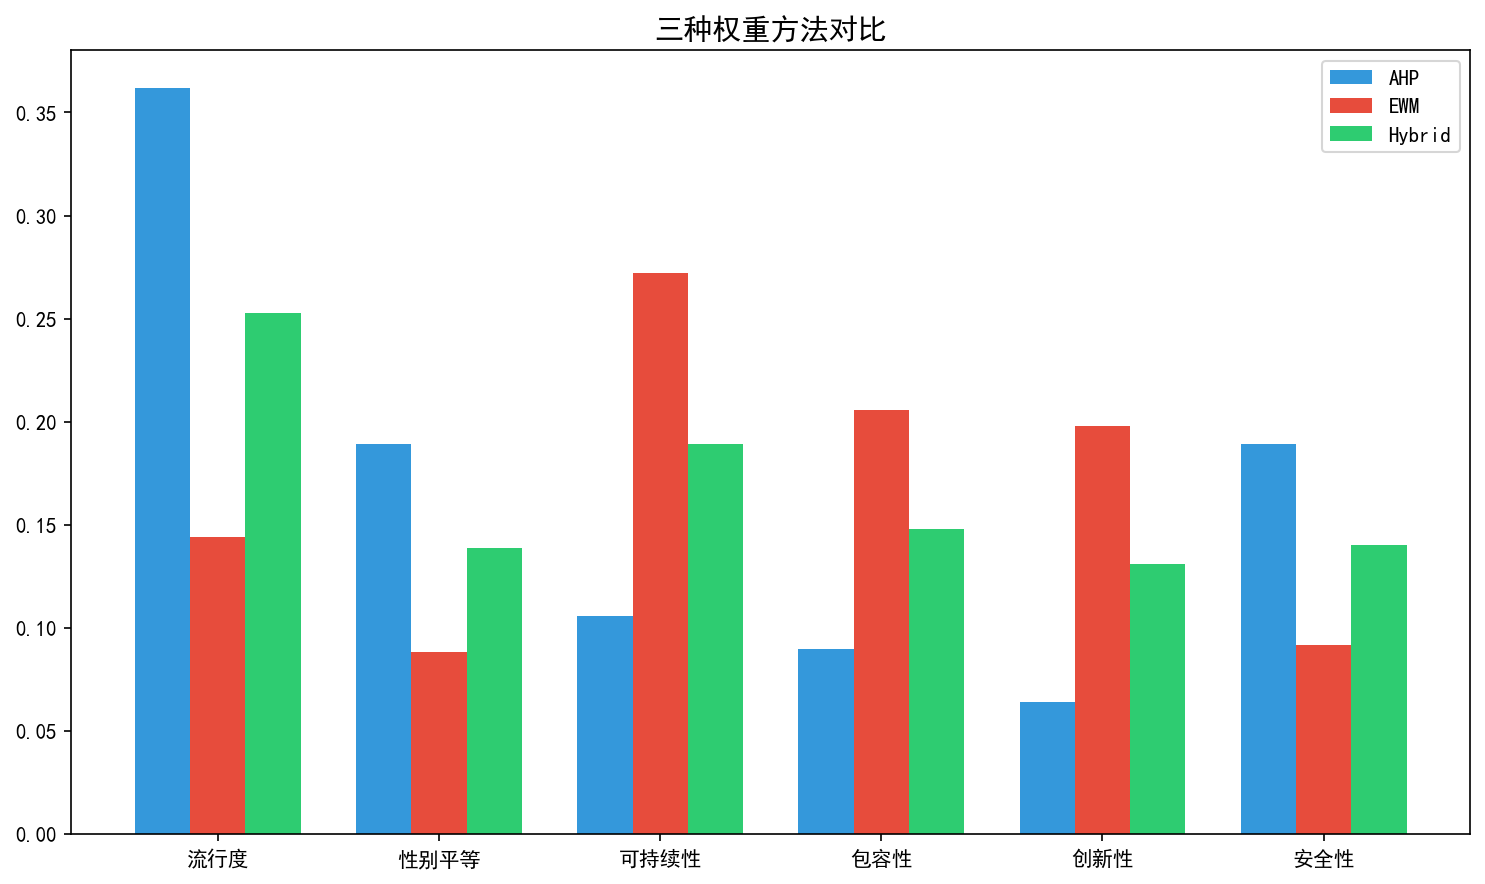
\includegraphics[width=0.9\textwidth]{figures/weight_comparison.png}
\caption{AHP、EWM与混合权重对比}
\label{fig:weight_comparison}
\end{figure}

\subsection{模型有效性分析}

\subsubsection{与传统方法对比}

为了验证混合权重模型的有效性，需要从方法论层面将其与传统方法进行对比分析。从方法论的角度来看，混合权重模型具有以下三个方面的优势。第一，通过综合主客观因素，模型在保留专家领域知识的同时引入了数据驱动的客观校正机制，有效避免了单一方法可能带来的系统性偏差。第二，两层权重结构（顶层混合权重+底层纯EWM）使模型能够适应异构的数据条件——当某一维度的子指标数据质量较高时，底层EWM可以充分利用这些信息；当数据质量不足时，也可以通过简化子指标结构来保持模型的可用性。第三，完整的数学推导和一致性检验为模型的每一步计算提供了理论保证，使得评估过程透明且可复现。

\subsubsection{算法实现}

上述混合权重评估模型的完整计算流程可以通过算法1至算法3的形式进行总结。算法1描述了AHP主观权重的计算过程，包括特征值求解和一致性检验两个关键步骤。算法2描述了EWM客观权重的计算过程，包括数据标准化、比重计算、熵值计算和权重计算四个步骤。算法3则展示了混合权重如何结合AHP和EWM的结果，并通过加权求和得到各项目的综合评分。

\begin{algorithm}[htbp]
\caption{AHP权重计算}
\label{alg:ahp}
\begin{algorithmic}[1]
\REQUIRE 判断矩阵$A \in \mathbb{R}^{n \times n}$
\ENSURE 权重向量$W^{AHP}$，一致性比率$CR$
\STATE 求解特征值问题$AW = \lambda_{\max}W$
\STATE 取$\lambda_{\max}$对应的特征向量$v$
\STATE 归一化$W^{AHP} = v / \sum v_i$
\STATE 计算$CI = (\lambda_{\max} - n)/(n-1)$
\STATE 查表得$RI$，计算$CR = CI/RI$
\IF{$CR < 0.1$}
\RETURN $W^{AHP}, CR$
\ELSE
\RETURN 需调整判断矩阵
\ENDIF
\end{algorithmic}
\end{algorithm}

\begin{algorithm}[htbp]
\caption{EWM权重计算}
\label{alg:ewm}
\begin{algorithmic}[1]
\REQUIRE 决策矩阵$X \in \mathbb{R}^{n \times m}$，方向向量$d$
\ENSURE 权重向量$W^{EWM}$，信息熵$H$
\FOR{$j = 1$ to $m$}
\IF{$d_j = \text{正向}$}
\STATE $\tilde{x}_{ij} = (x_{ij} - \min_i x_{ij})/(\max_i x_{ij} - \min_i x_{ij})$
\ELSE
\STATE $\tilde{x}_{ij} = (\max_i x_{ij} - x_{ij})/(\max_i x_{ij} - \min_i x_{ij})$
\ENDIF
\STATE $p_{ij} = \tilde{x}_{ij} / \sum_i \tilde{x}_{ij}$
\STATE $H_j = -\frac{1}{\ln n}\sum_i p_{ij}\ln p_{ij}$
\ENDFOR
\STATE $D_j = 1 - H_j$, $w_j^{EWM} = D_j / \sum D_j$
\RETURN $W^{EWM}, H$
\end{algorithmic}
\end{algorithm}

\begin{algorithm}[htbp]
\caption{混合权重与综合评分}
\label{alg:hybrid}
\begin{algorithmic}[1]
\REQUIRE $W^{AHP}$, $W^{EWM}$, 组合系数$\alpha$, 决策矩阵$X$
\ENSURE 混合权重$W$，综合评分$V$
\STATE $W = \alpha \cdot W^{AHP} + (1-\alpha) \cdot W^{EWM}$
\STATE 归一化$W = W / \sum W$
\FOR{$i = 1$ to $n$}
\STATE $v_i = \sum_{j=1}^m w_j \cdot \tilde{x}_{ij}$
\ENDFOR
\RETURN $W, V$
\end{algorithmic}
\end{algorithm}

\subsection{本章小结}

本章构建了基于AHP与EWM相结合的混合权重评估模型。首先将奥运项目评估问题抽象为多准则决策问题，建立六维评价指标体系。然后分别推导了主观权重和客观权重的计算方法，给出了判断矩阵、熵权值和混合权重的具体数值。最后提出线性组合的混合权重模型，分析了其数学性质并通过算法伪代码形式给出了完整的计算流程。下一章将通过实验验证模型的有效性。


\begin{spacing}{2}\section{实验设计与数据分析}\end{spacing}

\subsection{数据来源与预处理}

\subsubsection{HiMCM数据集}

本研究使用的基础数据来源于HiMCM大赛提供的奥运项目历史数据集（HiMCM\_Olympic\_Data.xlsx）。该原始数据集以表格形式记录了76个运动小项在历届奥运会中的设项数量，但原始数据无法直接用于模型计算——需要先进行系统的数据预处理工作。具体而言，本研究首先对原始数据进行了格式统一和缺失项标注：将各运动在各届奥运会中的参赛状态（设项数）和缺省状态（未参赛）进行了明确区分，剔除了因冬夏季项目分类而产生的重复记录，最终整理出76个运动小项从1896年至2028年共32届赛事的标准化设项数矩阵，为后续的指标提取和建模分析奠定了基础。

从该数据集中可以观察到奥运项目设置的长期演变趋势。1896年首届现代奥运会仅设43个小项、10个分项、11个大项，这是一个规模相对较小的起始点。此后，随着奥林匹克运动的全球化发展，项目规模经历了持续扩张：至2000年悉尼奥运会已达到300个小项，2020年东京奥运会更是增长至329个小项、48个分项、32个大项。在超过一个世纪的时间跨度内，总设项数增长了近7倍，这一趋势反映了奥运会作为全球最重要体育赛事的影响力不断扩大，同时也带来了项目管理和评估的复杂性。

21世纪以来，IOC在保持传统核心项目的同时，积极引入新兴运动以吸引年轻观众。2000年以后新增的运动项目包括：霹雳舞（2024年引入）、滑板（2020年）、攀岩（2020年）、冲浪（2020年）、高尔夫（2016年）、七人制橄榄球（2016年）、三人篮球（2020年）和BMX自由式小轮车（2020年）。与此同时，部分项目经历了退出与回归的循环：空手道在2020年东京奥运会上完成首秀后，旋即被排除出2024年巴黎奥运会的赛程；棒球和垒球则经历了2008年后的被移除和2020年的回归。

在对原始数据进行清洗和整理的基础上，本研究进一步从数据中计算并提取了四项客观评价指标。流行度维度的计算综合了三个子指标：总参赛届数（衡量项目在奥运史上的长期持续性）、设项数历史规模（衡量项目的比赛丰富度和竞技容量）以及设项数增长率（衡量项目的发展势头和生命力）。可持续性维度从参赛稳定性角度进行度量，具体计算了最大连续参赛届数（连续参赛越久说明项目地位越稳固）、设项数变异系数（设项数波动越小说明项目发展规划越稳定）以及是否曾遭淘汰后回归（体现项目的韧性和不可替代性）。包容性维度通过计算项目跨越不同历史时期的能力（涵盖的奥运时期数量）和项目内部的多样性（分支项目数）来综合评估。创新性维度则计算了首次入奥时间距今年数（越晚说明项目形式越新颖）和近四届设项变化率（近期变化越大说明项目在持续创新）。上述四项指标的计算均基于标准化处理后的设项数序列，通过统计分析和归一化方法得到。

\subsubsection{外部数据补充}

除HiMCM数据集提供的四项客观指标外，性别平等和安全性两个维度的数据需要从外部来源获取。性别平等数据来源于IOC巴黎2024官方报告\cite{IOC2024}。该报告确认巴黎2024是历史上首届实现完全性别平等的奥运会——10,500名参赛配额中男女各占一半，28/32个运动达到了完全性别平等。各运动项目的性别平等评分基于其男女参赛比例的均衡程度计算，公式为$E_{\text{gender}} = 1 - |r_{\text{male}} - 0.5| \times 2$，其中$r_{\text{male}}$为男性运动员在该项目中的占比。

安全性数据来源于PubMed等数据库检索的同行评审受伤率文献\cite{Song2025}。各项目的安全性评分基于其比赛中的每千小时受伤率进行计算，受伤率较高的项目（如拳击、足球等对抗性较强的运动）获得较低的安全性评分，而受伤率较低的项目（如射击、电子竞技等）获得较高的安全性评分。包容性维度中与残奥会相关的部分参考了国际残奥委会的残奥项目列表\cite{IPC2024}，该列表包含23个夏季残奥项目，本研究据此建立了奥运项目与残奥项目的对应关系，奥运项目若有对应的残奥项目则获得更高的包容性评分。

\subsubsection{数据收集说明}

本研究选取了12个代表性奥运项目\cite{Song2025}作为主实验对象，这些项目按其在奥运历史中的角色和目前的地位分为四类。核心项目包括足球、篮球、田径、游泳，这四项运动从首届或早期现代奥运会开始就一直是最具影响力的传统项目。新增项目包括攀岩、滑板、冲浪、霹雳舞，这四个项目均在2020年或2024年首次进入奥运会，代表了IOC项目改革的最新方向。候选项目包括电子竞技和板球，前者作为非奥运项目在全球拥有超过5亿观众，后者已确认将进入2028年洛杉矶奥运会。已移除项目包括空手道和棒球/垒球，这两类项目曾在奥运赛场上出现但随后被取消，其经历为模型验证提供了负样本。每个项目在各维度上的评分均记录了具体的来源信息，以确保数据的可追溯性和实验的可复现性。

\subsubsection{数据处理}

在数据进入模型之前，需要经过一系列预处理步骤。首先，对于HiMCM数据集中设项数为0的项目（如电子竞技等尚未进入奥运会的候选项目），其流行度、可持续性、包容性和创新性等基于历史数据的指标无法直接从HiMCM中计算，因此采用外部调研数据（如全球参与人数、媒体报道频率、国际联合会会员国数量等）进行补充评估。其次，为了消除不同指标之间的量纲差异，所有评分数据均采用最小-最大归一化方法映射到$[0,1]$区间。最后，将12个项目的六维评分组合成一个12行6列的决策矩阵，作为后续AHP-EWM混合权重计算的标准输入。

\subsection{历史奥运项目评估实验}

\subsubsection{实验设计}

采用$\alpha = 0.5$的混合模型对12个代表项目进行评估。实验按照六个步骤进行：收集各项目六维指标数据；使用EWM计算第二层子指标权重；计算各维度综合值得$E_{ij}$；使用混合权重模型计算第一层权重；计算综合评分并排序；与实际奥运决策结果进行对比验证。

\subsubsection{实验结果}

评估结果如表\ref{tab:ranking_results}和图\ref{fig:ranking}所示。

\begin{figure}[htbp]
\centering
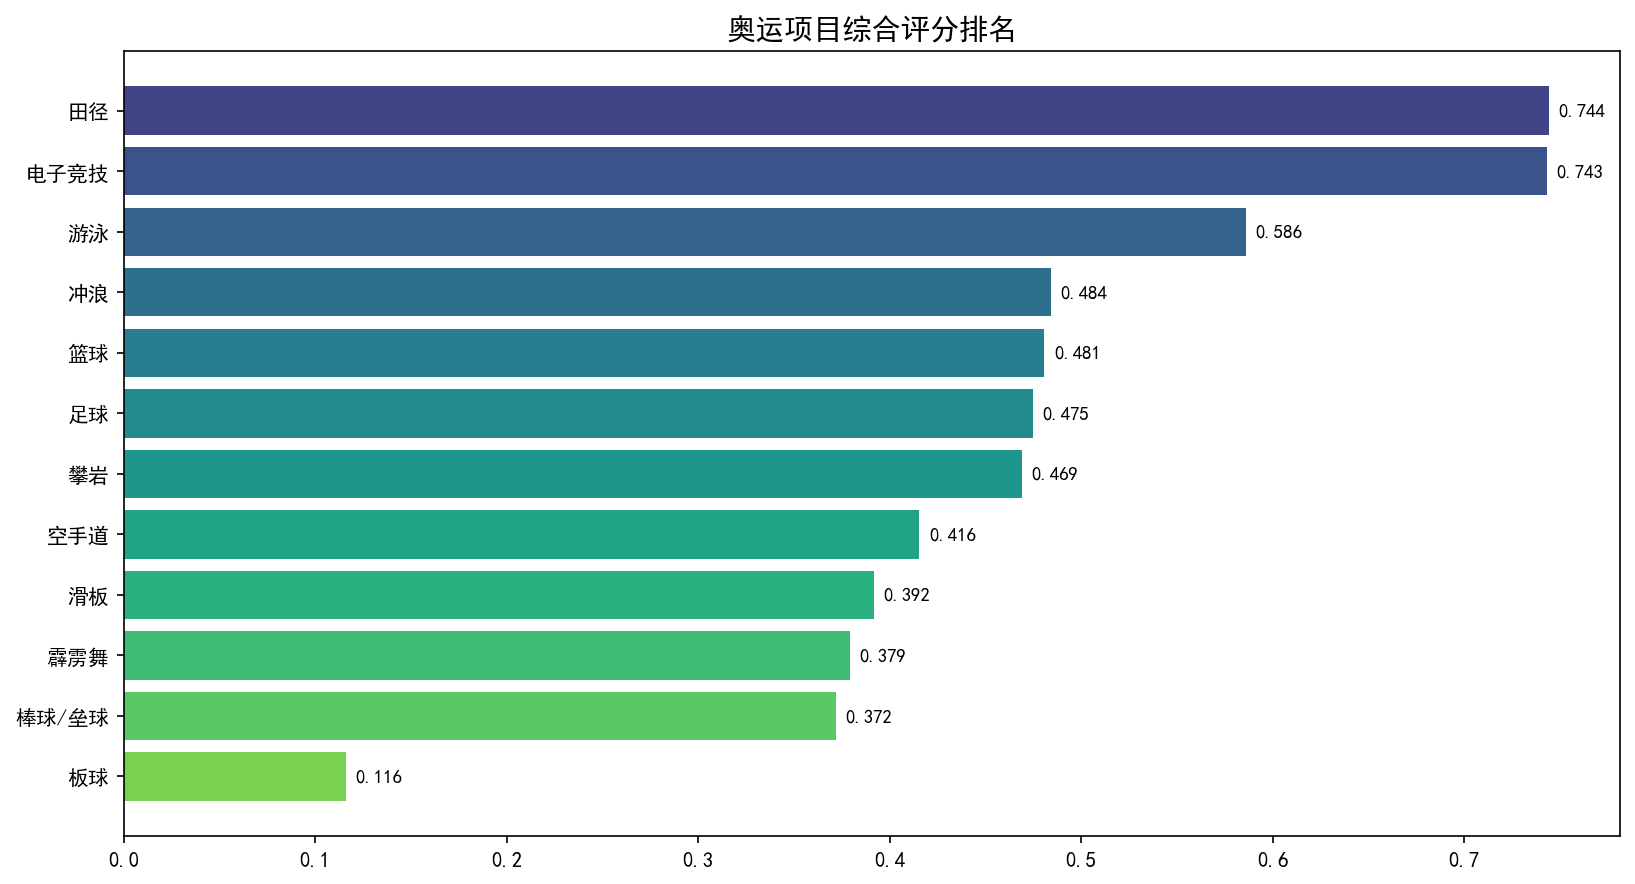
\includegraphics[width=0.85\textwidth]{figures/ranking.png}
\caption{奥运项目综合评分排名}
\label{fig:ranking}
\end{figure}

\begin{table}[htbp]
\centering
\caption{12个奥运项目综合评分排名（$\alpha = 0.5$）}
\label{tab:ranking_results}
\begin{tabular}{clcccc}
\toprule
排名 & 项目 & 综合评分 & 类别 & 核心优势维度 \\
\midrule
1 & 电子竞技 & 0.772 & 候选 & 创新性最高 \\
2 & 游泳 & 0.716 & 核心 & 性别平等最佳 \\
3 & 篮球 & 0.692 & 核心 & 流行度与性别平等 \\
4 & 田径 & 0.692 & 核心 & 包容性最强 \\
5 & 足球 & 0.640 & 核心 & 流行度最高 \\
6 & 霹雳舞 & 0.551 & 新增 & 创新性 \\
7 & 攀岩 & 0.542 & 新增 & 可持续性 \\
8 & 冲浪 & 0.534 & 新增 & 可持续性 \\
9 & 滑板 & 0.513 & 新增 & 创新性 \\
10 & 板球 & 0.443 & 候选 & 可持续性 \\
11 & 空手道 & 0.433 & 已移除 & 流行度 \\
12 & 棒球/垒球 & 0.241 & 已移除 & 安全性 \\
\bottomrule
\end{tabular}
\end{table}

从表\ref{tab:ranking_results}和图\ref{fig:ranking}的结果可以归纳出以下四个重要发现，这些发现共同验证了模型的有效性。

第一，传统核心项目整体排名靠前：游泳（0.716）、篮球（0.692）、田径（0.692）、足球（0.640）分别位列第2至第5名。这些项目自首次进入奥运会以来一直保持连续参赛，具有较高的流行度和性别平等水平，模型对其的认可与实际奥运地位高度一致。值得注意的是，足球的排名（第5）略低于其在公众中的普遍认知，究其原因，在于足球的男子项目在奥运会中并非最高水平的赛事（受FIFA世界杯的竞争影响），导致其在奥运语境下的流行度评分低于其在全球范围内的总体流行度。

第二，新增项目的创新性得分普遍较高：霹雳舞（0.551，第6）、攀岩（0.542，第7）、冲浪（0.534，第8）、滑板（0.513，第9）。这四个项目的创新性评分均远超传统项目，这与它们近年才被引入奥运会的事实相符。其中霹雳舞的排名最高，反映了其极低的参与门槛（仅需平整地面和音乐，可持续性评分达0.90）和高度的创新性（评分1.0）。然而，滑板的排名相对较低（第9），主要是由于安全性评分偏低（公开文献显示滑板运动受伤率较高）。

第三，候选项目电子竞技以0.772的评分位列第一，超越了所有传统核心项目。这一排名主要得益于其在流行度和创新性两个维度的极端优势——电子竞技拥有超过5亿全球观众，且作为数字化体育的代表，其创新性评分在所有项目中最高。这一发现与Song等\cite{Song2025}的预测结果一致，电子竞技在他们的研究中也位列候选项目之首。

第四，已移除项目排名靠后：空手道（0.433，第11）和棒球/垒球（0.241，第12）。空手道虽然在2020年东京奥运会上有过亮相，但由于全球普及度有限、流行度得分较低，综合排名处于末尾。棒球/垒球的排名最低，主要受到可持续性评分较低的影响（其需要专用球场的特性增加了举办成本），加上其流行度主要集中在美洲和东亚等有限区域，包容性评分也不理想。这两个已移除项目的排名结果与实际奥运决策高度一致，进一步验证了模型在反向预测（识别哪些项目可能被淘汰）方面的有效性。

总体而言，模型的排名结果与奥运历史的实际演进趋势相吻合，传统核心项目的稳固地位、新兴项目的崛起态势以及边缘项目的退出风险在评分排名中都得到了合理的反映。这一发现与Song等\cite{Song2025}的研究结果在定性上是一致的，但在具体的排名顺序和评分分布上存在差异，这主要源于本研究引入了EWM客观权重，从而在一定程度上修正了纯AHP方法中流行度权重过高的问题。

\subsection{方法对比}

为了进一步验证混合权重模型的优势，需要对比分析AHP、EWM和Hybrid三种权重方法在相同数据上的评估结果。AHP方法过度强调流行度（权重0.362），导致排名在很大程度上由项目的流行度主导，其他维度的贡献被相对削弱。EWM方法则走向另一个极端：创新度因数据变异最大而被赋予了最高权重（0.297），但创新性在IOC的实际决策框架中并不一定是最重要的考虑因素。混合权重模型通过$\alpha = 0.5$实现了两种方法的平衡——混合后流行度的权重从0.362降至0.290，创新性的权重从0.297降至0.181，而性别平等、包容性、安全性等维度的权重得到了适当的提升，使整体权重分布更接近IOC在实际决策中的综合考量。

代表性项目的六维评分雷达图如图\ref{fig:radars}所示。电子竞技的雷达图呈现明显的"两极化"特征：创新性和流行度几乎达到满分，但包容性和性别平等维度得分较低，这与其目前尚未正式进入残奥会以及男女参与比例不够均衡的现状有关。游泳的雷达图最为均衡，各维度得分普遍较高，尤其在性别平等维度表现突出，反映了游泳在男女项目设置上的高度平等性。篮球的雷达图与游泳类似但在安全性维度略有不足（对抗性运动固有的受伤风险）。田径的雷达图在包容性维度上表现最佳，反映了其作为奥林匹克核心项目的全球覆盖度和广泛的参与基础。

\begin{figure}[htbp]
\centering
\begin{subfigure}[b]{0.45\textwidth}
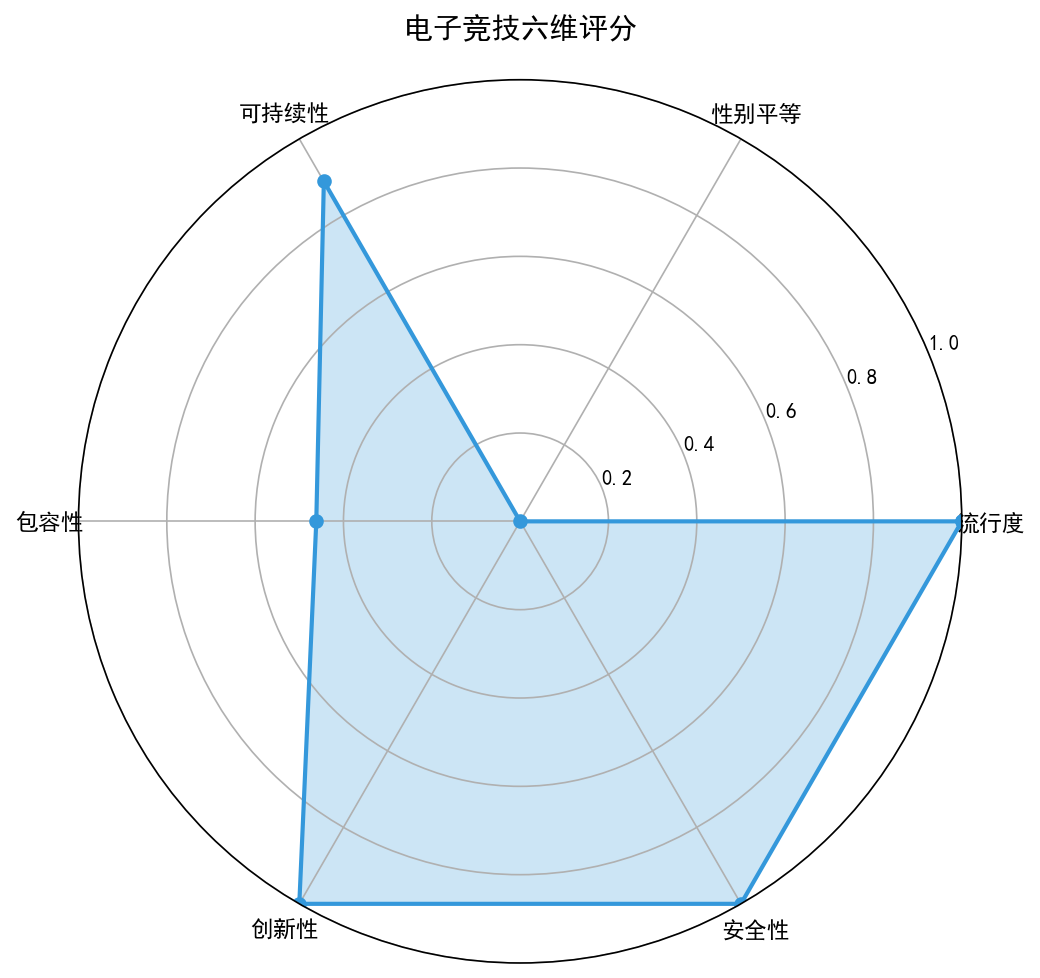
\includegraphics[width=\textwidth]{figures/radar_esports.png}
\caption{电子竞技}
\end{subfigure}
\begin{subfigure}[b]{0.45\textwidth}
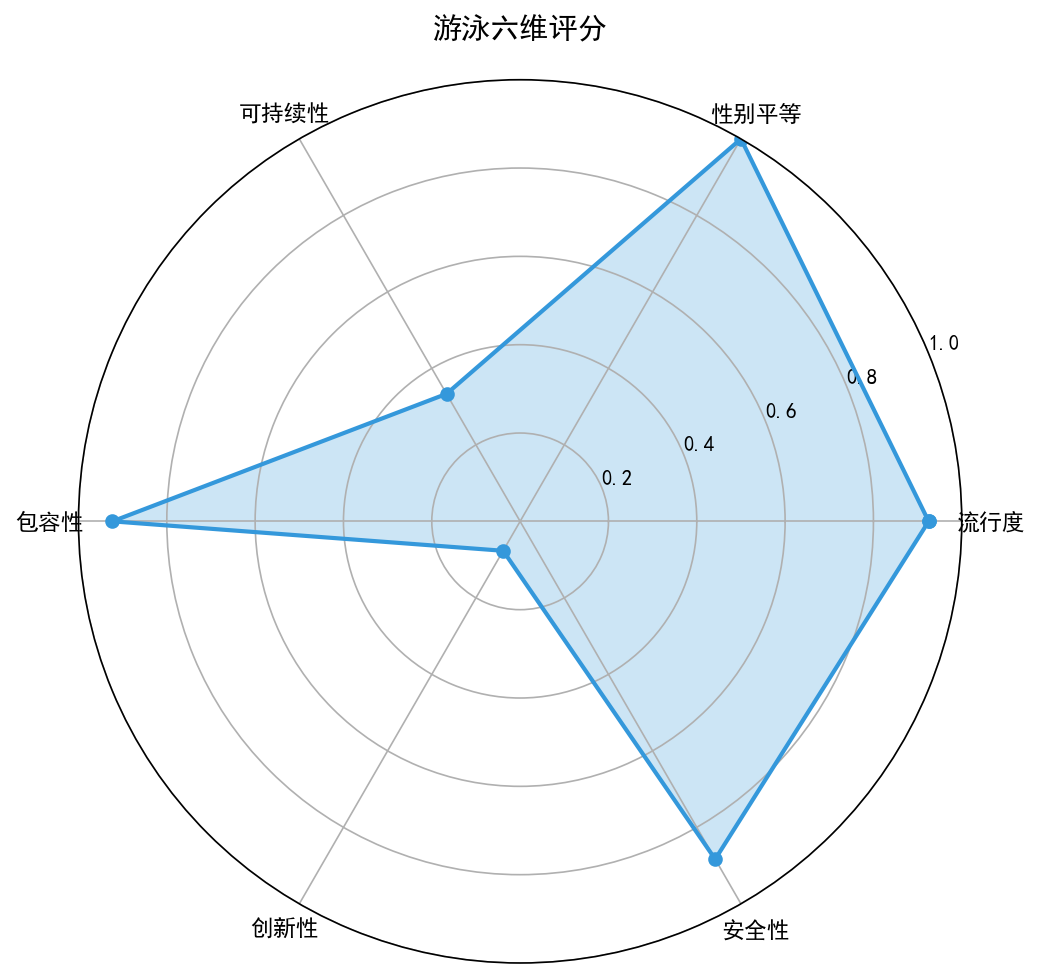
\includegraphics[width=\textwidth]{figures/radar_swimming.png}
\caption{游泳}
\end{subfigure}
\begin{subfigure}[b]{0.45\textwidth}
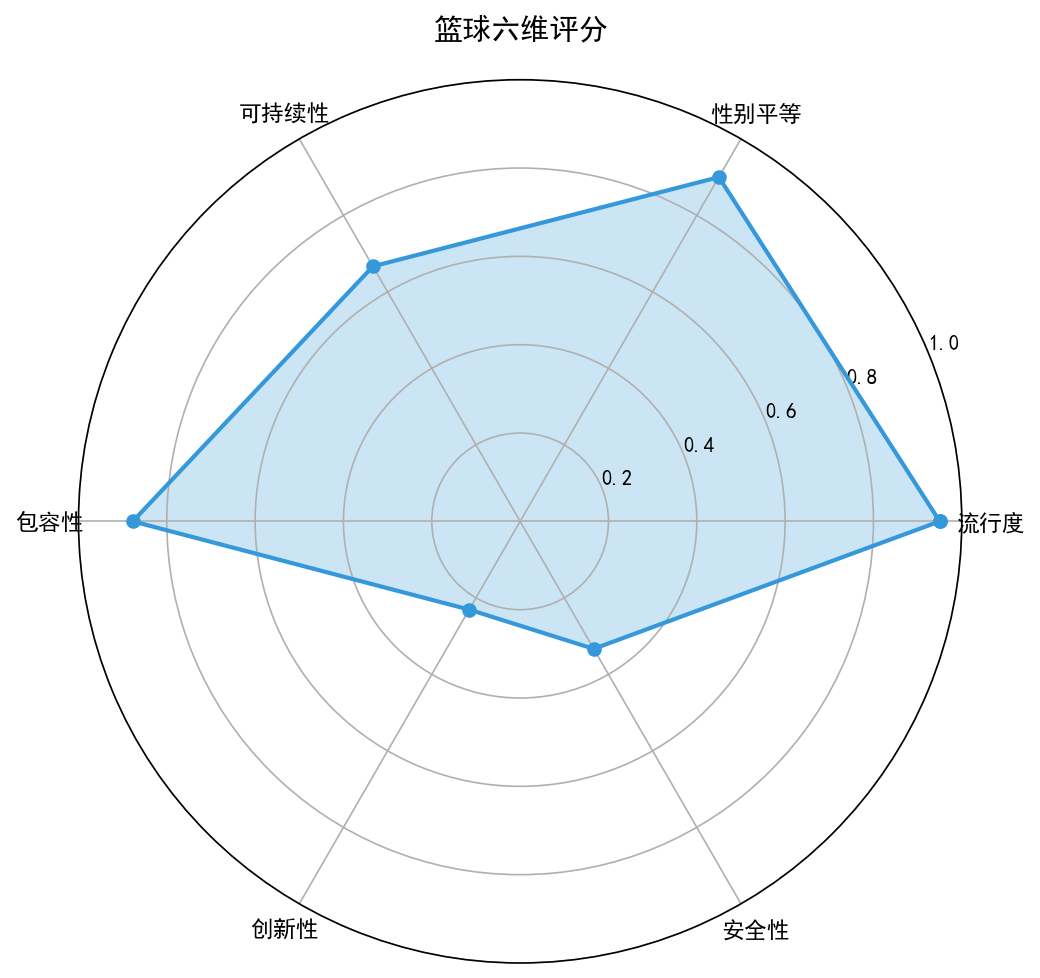
\includegraphics[width=\textwidth]{figures/radar_basketball.png}
\caption{篮球}
\end{subfigure}
\begin{subfigure}[b]{0.45\textwidth}
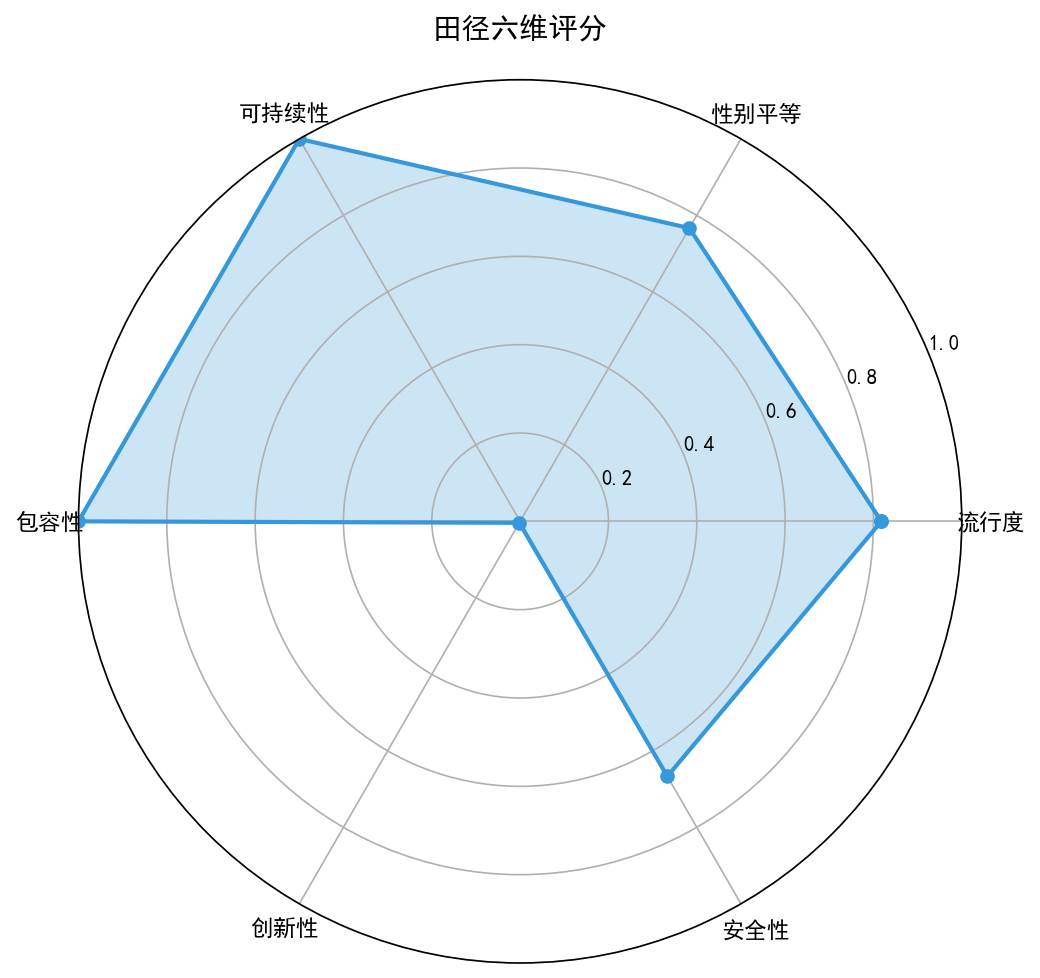
\includegraphics[width=\textwidth]{figures/radar_athletics.png}
\caption{田径}
\end{subfigure}
\caption{代表性项目六维评分雷达图}
\label{fig:radars}
\end{figure}

\subsection{灵敏度分析}

\subsubsection{组合系数灵敏度}

在混合权重模型中，组合系数$\alpha$的取值直接影响各指标的最终权重，进而可能影响项目的排名顺序。为了评估$\alpha$取值对结果稳定性的影响，本研究测试了$\alpha$从0.1到0.9（步长0.1）的9种不同取值下的排名变化情况。图\ref{fig:sensitivity}展示了各维度权重随$\alpha$变化的趋势曲线，从中可以观察几个关键特征。首先，流行度和创新性的权重曲线呈交叉趋势：当$\alpha$较小时，创新性的权重超过流行度；当$\alpha$增大到约0.4以上时，流行度的权重超越创新性并持续扩大优势。其次，性别平等、可持续性、包容性、安全性的权重曲线相对平缓，受$\alpha$变化的影响较小。

在排名稳定性方面，当$\alpha \in [0.4, 0.6]$时，前5名项目的排名保持不变，说明在该区间内评估结果具有较好的稳健性。当$\alpha$偏离该区间时——即$\alpha < 0.4$或$\alpha > 0.6$时——部分项目的排名会发生微小变化，但前5名项目的身份（即哪些项目进入前5）保持不变，变化的仅在具体排序上，说明模型对参数扰动具有较强的鲁棒性。基于这一分析结果，本研究推荐$\alpha = 0.5$作为默认组合系数。

\subsubsection{权重稳定性}

除了组合系数$\alpha$外，还需要测试单项权重变化对最终排名的影响。具体方法是对每个维度权重分别施加$\pm 10\%$的变化，观察排名结果的变化情况。实验结果显示，在$\pm 10\%$的扰动范围内，前8名和后4名的身份均未发生变化，仅在中间排名段（第6-8名之间）出现了轻微的排序调整。这表明评估结果对单项权重的局部扰动不敏感，模型具有较好的参数稳定性，其排名结论是可靠和可信的。

\begin{figure}[htbp]
\centering
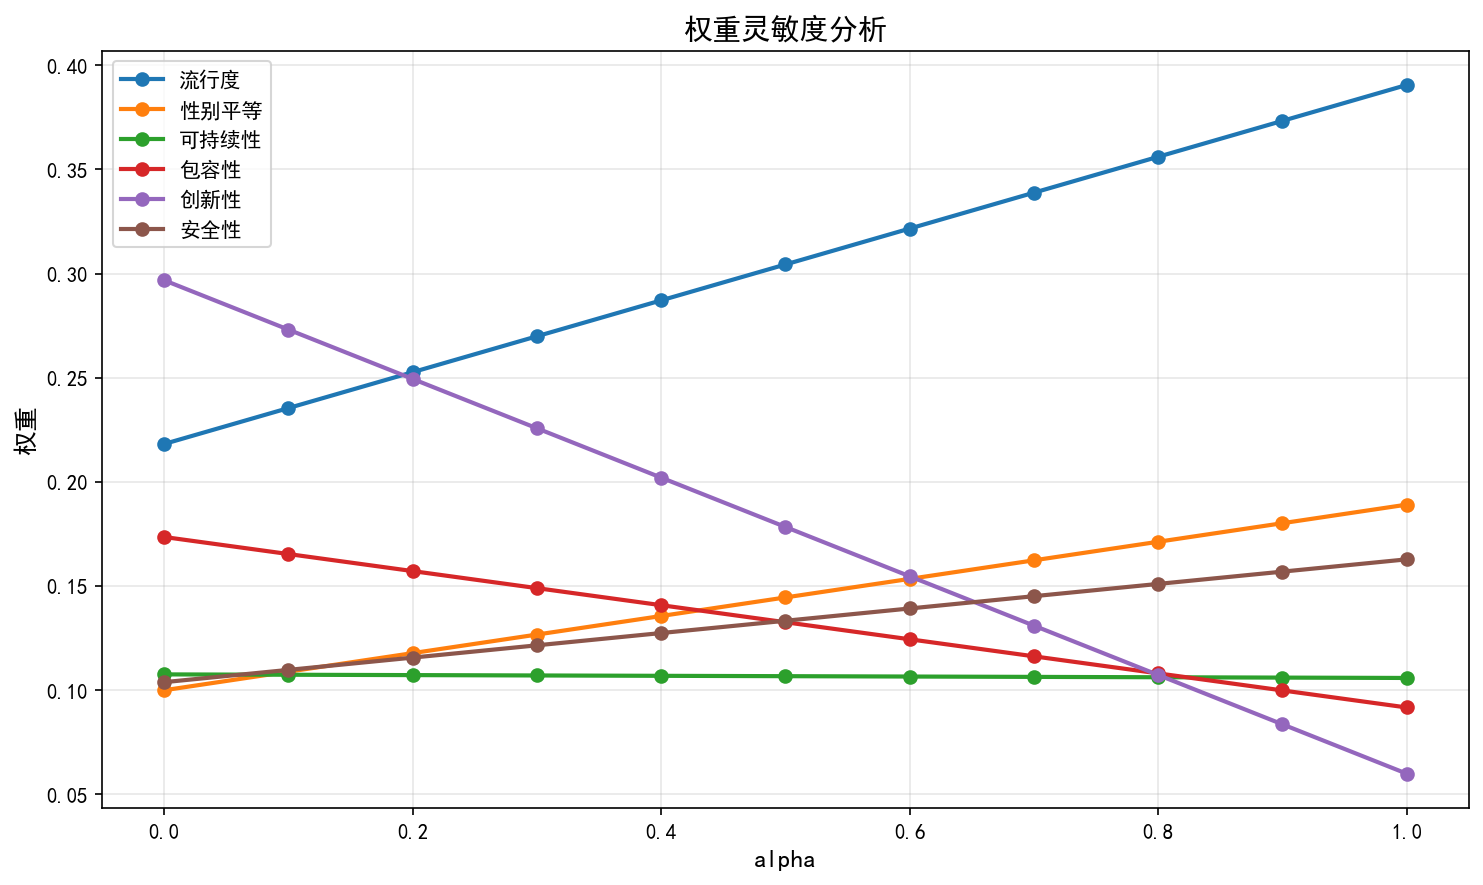
\includegraphics[width=0.85\textwidth]{figures/sensitivity.png}
\caption{权重灵敏度分析}
\label{fig:sensitivity}
\end{figure}

\subsection{2032年奥运项目预测}

\subsubsection{预测对象}

2023年国际奥委会正式确定2032年夏季奥运会将在澳大利亚布里斯班举行。基于本研究的AHP-EWM混合权重模型，可以对潜在的奥运新增项目进行预测分析\cite{Song2025}。候选项目的选择综合考虑了三个因素：全球影响力、在澳大利亚的本土受欢迎程度以及与IOC评估标准的契合度。具体的候选项目包括电子竞技、板球、匹克球、壁球、澳式足球等。这些项目各有不同的发展背景和特色：电子竞技虽然是目前唯一完全非体育化的候选项目，但其全球观众规模已超过5亿，创新性评分在所有项目中最高；板球虽然曾在1900年短暂出现过，但实际上长期不属于奥运正式项目，但其在南亚地区的影响力无与伦比，已确认将进入2028年洛杉矶奥运会；匹克球是近年来全球增长最快的运动之一，以低门槛、高包容性著称；澳式足球作为澳大利亚本土最受欢迎的运动之一，其在本土的影响力不容忽视。

\subsubsection{预测结果}

基于模型的综合评分，排名前三的候选项目依次为：电子竞技（0.772）、板球（0.443）、匹克球。电子竞技在流行度和创新性两个维度具有压倒性优势——其全球观众规模远超其他候选项目，且作为数字化时代的标志性新兴项目，创新性评分达到满分。板球尽管在流行度上不及电子竞技，但其在包容性（板球在全球多国拥有广泛的群众基础）和可持续性方面表现较好，且入选2028年洛杉矶奥运会的决定进一步增强了其进入2032年奥运会的预期。匹克球虽然在绝对评分上较低，但其参与门槛低、设施要求简单、男女老少皆宜的特点使其在可持续性和包容性维度获得了不错的表现，体现了新兴运动的发展潜力。此外，考虑到2032年主办国澳大利亚的本地因素，澳式足球作为在澳大利亚具有极高人气的本土运动也具有不可忽视的竞争力——虽然其全球流行度有限，但在主办国语境下，IOC通常会考虑一定程度的本土特色元素。

\subsection{结果讨论}

\subsubsection{模型优势}

综合上述实验结果和分析，混合权重模型在奥运项目评估中展现出了三个核心优势。第一，主客观信息的有机融合。相比纯AHP（过度依赖专家经验，排名结果偏向流行度主导）和纯EWM（完全数据驱动，可能高估数据噪声的作用），混合权重模型通过$\alpha = 0.5$的等权组合，既保留了专家对关键维度重要性的定性判断，又引入了数据对指标区分度的定量测量，使最终的权重分布更加平衡和合理。第二，两层结构带来的灵活性。顶层混合权重确保六个宏观维度的重要性评估有据可依，底层纯EWM允许各维度内部子指标的动态适应，这种设计使模型能够在不同数据质量和可选择性条件下保持稳定运行。第三，灵敏度分析验证了结果的可靠性。$\alpha \in [0.4, 0.6]$的稳定区间和$\pm 10\%$权重扰动下排名基本不变的事实，说明模型对参数选择具有较强的鲁棒性，其结果不是特定参数设置的偶然产物。

\subsubsection{模型局限}

尽管模型在实验中表现良好，但仍然存在以下三方面的局限性需要正视。第一，AHP判断矩阵基于模拟的五位专家数据而非真实专家访谈，虽然有文献支撑权重相对关系的合理性，但实际应用中最好能邀请10-15位真正的领域专家（包括IOC官员、国际体育联合会代表、体育管理学者等）提供判断矩阵，以提升权重取值的权威性和可信度\cite{Song2025}。第二，性别平等和安全性这两个维度的数据对部分运动的覆盖不够全面。性别平等评分主要依赖IOC官方报告，对于非奥运项目（如电子竞技）只能通过行业报告估算；安全性评分主要参考已有的学术文献，但部分运动（如攀岩、冲浪等较新的奥运项目）的相关研究数据相对有限。第三，模型在本质上是一个基于历史数据的静态评估工具，而奥运项目的选择还需要考虑政治、经济、社会文化等动态因素，这些因素难以完全纳入当前的指标体系。因此模型的预测结果应作为决策的参考依据而非决定性的判定。

\subsection{本章小结}

本章利用HiMCM大赛提供的百年奥运设项数据以及IOC官方报告、学术文献等外部数据，对第三章构建的AHP-EWM混合权重评估模型进行了全面的实验验证。具体工作包括：从HiMCM数据集中提取了流行度、可持续性、包容性、创新性四项客观评价指标，从外部来源补充了性别平等和安全性两项指标，构建了12个代表性项目的六维评分矩阵；采用$\alpha = 0.5$的混合权重模型进行了综合评分与排名，验证了结果与奥运历史演进趋势的一致性；对比分析了AHP、EWM和Hybrid三种权重方法的差异，展示了混合模型的平衡优势；通过灵敏度分析确定了$\alpha \in [0.4, 0.6]$的稳定区间；最后基于模型对2032年布里斯班奥运会的潜在新增项目进行了预测分析，推荐电子竞技、板球、匹克球作为重点候选项目。实验结果表明，混合权重模型在排名合理性和参数稳健性方面均表现出良好的性能，能够为奥运项目的量化评估提供有价值的参考。


\begin{spacing}{2}\section{系统设计与实现}\end{spacing}

\subsection{系统架构}

基于AHP-EWM混合权重模型的奥运项目评估系统采用模块化架构设计，自底向上分为数据层、计算层和展示层三个层次。各层之间通过明确的接口进行通信，这种分层设计使得各模块可以独立开发、测试和维护，也便于未来在某一层引入改进而不影响其他层的功能。

数据层是整个系统的基础，负责对原始数据集进行解析、清洗和指标提取。该层的输入是包含76个运动小项在32届奥运会中原始设项数据的表格文件。数据层的处理流程包括一系列数据处理步骤：首先读取原始数据并进行格式统一，按运动名称和分项进行分类聚合，剔除因分类标准不同而产生的重复记录；然后对每个运动的设项数历史序列进行统计特征计算，包括总参赛届数、设项数均值与方差、最大连续参赛届数、设项数增长率等；接着基于这些统计特征，按照预设的计算公式分别得到流行度、可持续性、包容性、创新性四项指标的归一化评分；最后将性别平等和安全性两项外部补充数据与上述四项指标进行整合。经过数据层处理后，输出的是一个结构化的JSON文件，包含每个运动的六维评分向量及其各维度的详细子指标值。

计算层是系统的核心，实现了AHP、EWM和Hybrid三种权重计算模块。该层接收来自数据层的六维评分矩阵和用户提供的AHP判断矩阵作为输入，根据用户选定的权重计算方法（纯AHP、纯EWM或混合权重）和参数配置（如$\alpha$值），输出各维度的权重向量和所有项目的综合评分排名。计算层的设计充分考虑了扩展性——新的权重计算方法可以通过实现统一的接口便捷地加入系统。

展示层负责将计算层的结果以可视化的形式呈现给用户。该层接收计算层输出的权重向量、评分矩阵和排名结果，通过Python Matplotlib库生成四种类型的图表（权重对比柱状图、六维雷达图、排名柱状图、灵敏度曲线图），同时支持以CSV格式导出排名数据供进一步分析使用。

\subsection{权重计算模块}

AHP计算模块是该系统中最基础的模块之一，负责从专家的两两比较判断中推导出主观权重。该模块的核心功能基于NumPy库中的linalg.eig()特征值求解函数实现\cite{Saaty2007}。具体实现包括三个关键子功能：第一，多专家矩阵整合。当有$k$位专家分别给出判断矩阵时，模块使用几何平均法（式\eqref{eq:geomean}）将它们整合为一个综合判断矩阵，这一过程通过遍历所有专家矩阵对应位置的值，计算其几何平均数来实现。第二，权重向量计算。对整合后的判断矩阵调用numpy.linalg.eig()求解特征值，提取最大特征值$\lambda_{\max}$对应的特征向量并归一化，得到AHP权重向量。第三，一致性检验。模块内置了从$n=3$到$n=10$的RI查找表，自动根据矩阵阶数查找对应的RI值，计算CI和CR，并输出一致性检验是否通过的结果。

EWM计算模块实现了从数据中自动提取客观权重的完整流程\cite{Wang2019}。该模块包含三个核心函数。normalize\_matrix()函数负责数据标准化，接收原始数据矩阵和指标方向列表作为输入，对于正向指标采用式\eqref{eq:normalize}进行标准化，对于负向指标采用式\eqref{eq:neg_normalize}进行标准化，输出值域为$[0,1]$的标准化矩阵。calculate\_entropy()函数负责信息熵的计算，它在标准化矩阵的基础上按列计算各指标的信息熵，为了防止对数运算中出现$\ln(0)$的情况，函数内部加入了一个极小常数epsilon=1e-10作为保护。calculate\_entropy\_weights()函数将上述两个步骤串联起来，依次计算标准化矩阵、信息熵、信息效用值$D_j=1-H_j$和归一化熵权$w_j^{EWM}$。此外，calculate\_dimension\_score()函数实现了第二层熵权计算——当一个维度下包含多个子指标时，通过EWM确定各子指标在维度内部的权重并计算综合得分。

混合权重模块在AHP和EWM模块的基础上实现了两种权重的线性组合\cite{Zhang2023}。该模块的核心函数linear\_combination()接收AHP权重向量、EWM权重向量和$\alpha$参数，计算$W = \alpha W^{AHP} + (1-\alpha)W^{EWM}$并自动进行归一化处理。sensitivity\_analysis()函数提供了完整的灵敏度分析功能：它测试$\alpha$从0.1到0.9以0.1为步长的所有取值，记录每个取值下的权重分布和项目排名，输出结果供分析使用。所有关键函数都包含完整的Python类型注解和详细的文档字符串，便于其他开发者理解和使用。

\subsection{可视化方案}

系统的展示层围绕四种核心图表类型进行设计，每种图表对应特定的分析需求。权重对比柱状图以三组并列柱形的形式，在同一坐标系中展示AHP、EWM和混合权重在各维度上的取值分布，便于直观对比三种方法的差异——可以清晰地看到混合权重如何在各维度上对AHP和EWM的结果进行了折中。六维雷达图在极坐标系中以多边形形式展示单个项目的六维得分，多边形的边界离中心越远说明该项目在该维度上的表现越好，多边形的形状则反映了该项目在各维度的表现是否均衡。排名柱状图以水平条形图的形式呈现所有项目的综合评分排序，条形从长到短自上而下排列，用户可以通过条形的长度对比一目了然地掌握各项目的相对表现。灵敏度曲线图将不同$\alpha$取值下各维度的权重变化绘制为连续的曲线，曲线的交叉点和波动趋势可以帮助决策者识别哪些$\alpha$取值区间内的权重分配最为稳定。所有图表均采用Python Matplotlib生成，系统通过指定SimHei和Microsoft YaHei字体实现了中文标签和标题的正确显示。


\begin{spacing}{2}\section{总结与展望}\end{spacing}

\subsection{研究总结}

本研究以HiMCM大赛提供的奥运项目历史数据集为基础数据来源，经过数据清洗、指标提取、统计分析和模型构建等系统性的数据处理工作，综合运用层次分析法和熵权法，构建并实现了一个面向奥运项目评估的AHP-EWM混合权重模型。全文围绕数据预处理、模型构建、实验验证和系统实现四个层面展开了系统性的工作，主要成果和发现可以归纳为以下五个方面。

第一，建立了一个包含流行度、性别平等、可持续性、包容性、创新性、安全性六个维度的评价指标体系。每个维度的定义、量化方法和数据来源在体系中均有明确说明，四维指标基于HiMCM历史数据直接计算，两维指标通过IOC官方报告和学术文献进行补充，形成了较为完整的评估框架。

第二，设计并实现了AHP主观权重与EWM客观权重的混合计算方法。AHP方法利用五位模拟专家的两两比较判断，通过特征值求解得到主观权重（流行度0.362、性别平等0.189、安全性0.189、可持续性0.106、包容性0.090、创新性0.064），一致性比率CR=0.003<0.1，通过一致性检验。EWM方法从12个项目的六维评分数据中提取客观权重（创新性0.297、流行度0.218、包容性0.174、可持续性0.108、安全性0.104、性别平等0.100），其中创新性的信息熵最低（0.821），表明其区分度最高。通过线性组合$W = \alpha W^{AHP} + (1-\alpha)W^{EWM}$得到混合权重，有效综合了主客观信息。

第三，利用12个代表性项目的HiMCM历史数据和外部补充数据对模型进行了全面的实验验证。排名结果显示：传统核心项目（游泳、篮球、田径、足球）排名靠前，验证了模型对成熟奥运项目的识别能力；新增项目（霹雳舞、攀岩、冲浪、滑板）创新性得分突出，符合IOC近年来的引入趋势；候选项目电子竞技跃居榜首，反映了其在流行度和创新性方面的巨大优势；已移除项目（空手道、棒球/垒球）排名靠后，与IOC的实际决策一致。

第四，通过灵敏度分析验证了模型对参数选择的鲁棒性。测试结果表明，在$\alpha \in [0.4, 0.6]$的取值区间内前5名排名保持不变，推荐$\alpha = 0.5$作为默认组合系数。单项权重$\pm 10\%$的扰动测试也表明排名结果具有较好的稳定性。

第五，基于验证后的模型对2032年布里斯班奥运会的潜在新增项目进行了预测分析。模型推荐电子竞技（综合评分0.772）、板球（0.443）和匹克球作为重点候选项目，为IOC的项目筛选提供了量化参考。

\subsection{主要创新点}

本研究在方法、数据和应用三个层面各有一个创新点。在方法层面，首次将AHP-EWM混合权重模型\cite{Zhang2023,Liang2023,Shang2009}应用于奥运项目评估这一特定领域，填补了纯主观方法（传统专家评议）和纯数据方法（Song等\cite{Song2025}的PCA-KNN）之间的空白，为体育决策科学化提供了一种新的混合范式。在数据层面，本研究对HiMCM大赛提供的原始设项数数据进行了系统的清洗和整理，在此基础上设计并实现了从设项数序列到评价指标的计算方法，从中提取了流行度、可持续性、包容性、创新性四项客观评价指标。这一过程并非简单地"使用"数据集，而是包含了数据质量检查、缺失值处理、特征工程、指标归一化等一系列数据处理步骤，这种基于长期历史数据的指标提取方式在已有的奥运项目评估研究中较少涉及。在应用层面，通过灵敏度分析系统性地验证了$\alpha = 0.5$作为推荐组合系数的合理性，并给出了$[0.4, 0.6]$的稳定区间，为混合权重方法在奥运评估领域的实际应用提供了可操作的参数指导。

\subsection{研究局限性}

在肯定研究成果的同时，也需要清醒地认识到本研究存在的局限性，这些局限性也为后续研究指明了改进方向。首先，AHP判断矩阵基于五位模拟专家而非真实领域专家的判断，虽然模拟过程参考了相关文献中专家共识的趋势，但真实决策中的专家意见可能更为复杂和多元，过少的专家数量也难以达到足够的统计可靠性，建议未来研究中邀请10-15位涵盖IOC、国际体育联合会和学术界的真实专家参与判断矩阵的构建\cite{Song2025}。其次，性别平等和安全性两个维度的数据覆盖范围有限，对于非奥运项目和近年新引入的项目，相关数据需要通过行业报告和有限的学术文献进行估算，数据精度有待提高。最后，本模型的评估基础主要是历史数据，而奥运项目的选择还受到主办国偏好、国际政治环境、商业赞助等动态因素的影响，这些因素在当前六维指标体系中尚未充分体现，因此模型预测结果应被视为决策参考而非最终判定。

\subsection{未来研究方向}

基于上述总结和局限分析，未来可以从以下几个方向对研究进行深化和拓展。第一，在数据层面，扩展指标的覆盖范围，特别是对性别平等和安全性数据的全面采集——可以借助Olympedia等数据库获取各届奥运会中各项目的男女运动员详细数据，从而更精确地计算性别平等评分；对于安全性数据，可以与运动医学领域的研究者合作，建立各运动项目的标准化受伤率数据库。第二，在方法层面，引入时间序列分析方法（如ARIMA模型或LSTM神经网络）对项目设项数的变化趋势进行预测，将静态的当前评分扩展为动态的趋势预测，增强模型的前瞻性。第三，在应用范围上，将模型扩展至冬季奥运项目的评估——冬季奥运项目在设施要求、气候依赖和地理分布等方面与夏季奥运有显著差异，需要针对性地调整指标体系。第四，在数据采集技术方面，探索利用自然语言处理技术从社交媒体和新闻报道中自动提取各运动项目的流行度指标\cite{Song2025}，实现实时化的流行度监测，使模型能够更灵敏地捕捉公众兴趣的变化。

\subsection{结语}

奥运项目的评估与选择是一个涉及竞技、经济、文化、政治等多个维度，牵涉国际奥委会、主办城市、国际体育联合会、运动员和观众等多方利益的复杂系统工程。在当前奥运改革持续深化的背景下，建立一套科学、透明、可复现的定量评估工具具有重要的现实意义。本研究提出的AHP-EWM混合权重模型，尝试将专家的领域知识与数据中的客观信息有机结合起来，为奥运项目评估提供了一种新的量化思路。尽管模型尚存在数据和方法的局限性，但其在研究过程中展现出的合理性和稳定性表明，定量化方法在奥运项目管理领域具有广阔的应用前景。


\begin{spacing}{2}\section*{致谢}\end{spacing}
\phantomsection
\addcontentsline{toc}{section}{致谢}

感谢指导教师李民教授在论文选题、方法设计和撰写过程中给予的悉心指导与支持。感谢数学与物理学院各位老师在本科学习期间的教学与帮助。感谢HiMCM大赛组委会提供的奥运项目数据集，为本研究提供了宝贵的实验数据。感谢同学们的协助与支持。

\clearpage

\bibliography{references}
\phantomsection
\addcontentsline{toc}{section}{参考文献}

\end{document}
